\documentclass[openany]{book}
\usepackage[utf8]{inputenc}
\usepackage[spanish]{babel}
\usepackage{geometry}
 \geometry{
 a4paper,
 total={170mm,257mm},
 left=20mm,
 top=20mm,
 }
\usepackage{graphicx}
\usepackage{titling}
\usepackage[hidelinks=true]{hyperref}
\usepackage{amsmath}
\usepackage{amssymb}
\usepackage{amsthm}
\usepackage{mdframed}
\usepackage[usenames,dvipsnames]{xcolor}
\usepackage{verbatim}
\usepackage{marginnote}
\usepackage{background}
\usepackage[most]{tcolorbox}
\usepackage{tikz}
\usetikzlibrary{calc} 
\usepackage{varwidth}
\usepackage{pifont}
\usepackage{minitoc}
\usepackage[rflt]{floatflt}
\usepackage{listings}
\usepackage{titlesec}
\usepackage{tabularx}
\usepackage{array}
\usepackage{colortbl}
\tcbuselibrary{skins}
\usepackage{multicol}
\usepackage{subcaption}
\usepackage{empheq}
\usepackage{tikz}

\backgroundsetup{
    scale=5,
    color=gray!40,          % Color gris claro
    opacity=0,
    angle=45,
    position=current page.center,
    contents={Sistemas Operativos - FaMAF 2024}
}
\titleformat{\chapter}
  {\normalfont\huge\bfseries} % formato del título
  {} % sin etiqueta (elimina "Capítulo X")
  {0pt} % separación entre la etiqueta y el título
  {} % sin código adicional antes del título

\titlespacing{\chapter}
  {0pt} % indentación izquierda
  {0pt} % espacio vertical antes
  {15pt} % espacio vertical después

\newcolumntype{Y}{>{\centering\arraybackslash}X}
  \tcbset{tab2/.style={enhanced,fonttitle=\bfseries,fontupper=\normalsize\sffamily,
  colback=white!10!white,colframe=red!50!black,colbacktitle=Salmon!40!white,
  coltitle=black,center title}}

\newcolumntype{Y}{>{\centering\arraybackslash}X}
  \tcbset{tab3/.style={enhanced,fonttitle=\bfseries,fontupper=\normalsize\sffamily,
  colback=white!10!white,colframe=blue!50!black,colbacktitle=blue!40!white,
  coltitle=black,center title}}

\definecolor{darkcyan}{HTML}{0091A4}
\definecolor{brightcyan}{HTML}{dcf0f2}  
\newmdenv[
    topline=false,
    rightline=false,
    bottomline=false,
    leftline=true,
    linecolor=darkcyan,
    linewidth=3pt,
    backgroundcolor=brightcyan,
    frametitle=Respuesta
]{rta}

\usepackage{fancyhdr}
\pagestyle{fancy}
\fancyhf{}
\lhead{Pedro Villar}
\rhead{-----------}

\lfoot{Sistemas Operativos 2024}
\rfoot{\thepage}
% \renewcommand{\mtctitle}{\section*{Índice de Sección}}

\newtcolorbox[auto counter, number within=section]{exercise}[2][]{%
    colback=gray!15!black,      % Fondo oscuro suave
    colframe=gray!50!black,     % Borde oscuro suave
    coltitle=white,             % Color del título
    fonttitle=\bfseries,        % Título en negrita
    title=Ejercicio~\thetcbcounter: #2,
    enhanced,                   % Mejoras visuales
    sharp corners,              % Esquinas rectas
    boxrule=0.5pt,              % Grosor del borde
    #1                          % Otros parámetros opcionales
}



% ---- Cosas útiles ----
% Resaltado en azul
% \colorbox{blue!20}{}
% Resaltado con tcolorbox
% \myverb[color]{texto}

\NewTotalTCBox{\myverb}{ O{red} v !O{} } { fontupper=\ttfamily,nobeforeafter,tcbox raise base,arc=0pt,outer arc=0pt, top=0pt,bottom=0pt,left=0mm,right=0mm, leftrule=0pt,rightrule=0pt,toprule=0.3mm,bottomrule=0.3mm,boxsep=0.5mm, colback=#1!10!white,colframe=#1!50!black,#3}{#2}
\NewTotalTCBox{\commandbox}{ s v } 
{verbatim,colupper=white,colback=black!75!white,colframe=black} 
{\IfBooleanT{#1}{\textcolor{red}{\ttfamily\bfseries \$ }}% 
    \lstinline[language=command.com,keywordstyle=\color{blue!35!white}\bfseries]^#2^}

\begin{document}
\chapter{Notas de Clase - Concurrencia}

\begin{tcolorbox}[colback=black!5!white,colframe=black!75!black]
    Capítulos del OSTEP: 26, 27, 28, 30, 31, 32
\end{tcolorbox}

\section{Introducción}
Un \textit{programa multihilo} tiene más de un punto de ejecución (es decir, múltiples PCs, cada uno obteniendo y ejecutando instrucciones). Otra forma de verlo es que cada hilo es muy parecido a un proceso separado, con una diferencia: comparten el mismo espacio de direcciones y, por lo tanto, pueden acceder a los mismos datos.

El estado de un solo hilo es, por lo tanto, muy similar al de un proceso. Tiene un \textbf{contador de programa} (PC) que rastrea desde dónde el programa obtiene las instrucciones. 
\begin{itemize}
    \item Cada hilo tiene su propio conjunto privado de registros que utiliza para el cálculo; así, si hay dos hilos que se ejecutan en un solo procesador, al cambiar de ejecutar uno (T1) a ejecutar el otro (T2), debe realizarse un cambio de contexto.
    \item El cambio de contexto entre hilos es bastante similar al cambio de contexto entre procesos, ya que el estado de los registros de T1 debe guardarse y el estado de los registros de T2 restaurarse antes de ejecutar T2.
    \item Con los procesos, guardábamos el estado en un bloque de control de proceso (PCB); ahora necesitaremos uno o más bloques de control de hilos (TCBs) para almacenar el estado de cada hilo de un proceso. 
\end{itemize}

\begin{floatingfigure}[r]{0.5\textwidth}
    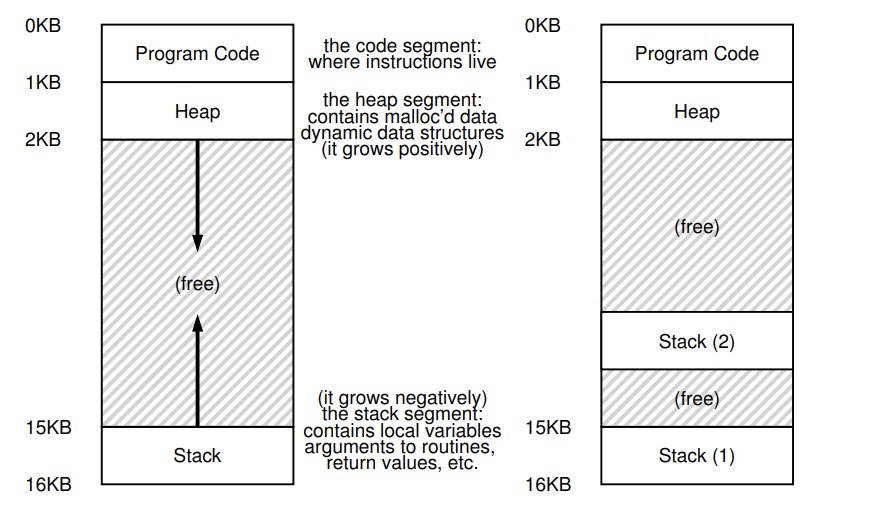
\includegraphics[width=0.5\textwidth]{src/multihilo.png}
    \caption{Stack de un proceso multihilo}
\end{floatingfigure}

Sin embargo, hay una diferencia importante en el cambio de contexto que realizamos entre hilos en comparación con los procesos: \textbf{el espacio de direcciones permanece igual} (es decir, \newline \colorbox{blue!20}{no es necesario cambiar la tabla de páginas}.

Otra diferencia importante entre hilos y procesos tiene que ver con la pila. En el módelo clásico, hay una sola pila, que reside en la parte inferior del espacio de direcciones. Sin embargo, en un proceso multihilo, \colorbox{blue!20}{cada hilo se ejecuta de forma independiente} y, por supuesto, puede llamar a varias rutinas para realizar el trabajo que esté haciendo. En lugar de una sola pila en el espacio de direcciones, \textbf{habrá una por cada hilo}.

\subsection{Ventajas de los hilos}
\begin{enumerate}
    \item \colorbox{blue!20}{Paralelismo:} si se tiene el programa que ejecute varias tareas, en un sistema con múltiples procesadores, es posible acelerar considerablemente este proceso utilizando los procesadores para \textbf{realizar cada uno una parte del trabajo}. La tarea de transformar tu programa estándar de un solo hilo en un programa que realiza este tipo de trabajo en múltiples CPUs se llama \colorbox{blue!20}{paralelización}.
    \item \colorbox{blue!20}{Evitar bloquear el progreso del programa debido a operaciones de entrada/salida (E/S) lentas}: usar hilos es una forma natural de evitar quedarse atascado; mientras un hilo en tu programa espera (es decir, está bloqueado esperando E/S), el planificador de la CPU puede cambiar a otros hilos que están listos para ejecutarse y hacer algo útil. El uso de hilos permite la superposición de E/S con otras actividades dentro de un solo programa.
\end{enumerate}

\subsection{Aspectos importantes y conceptos clave}
\begin{itemize}
    \item \myverb[blue]{Condición de carrera:} es un problema que surge cuando dos o más hilos intentan modificar una variable compartida al mismo tiempo. Los resultados dependen del momento en que se ejecuta el código. Con algo de mala suerte (es decir, cambios de contexto que ocurren en puntos inoportunos durante la ejecución), obtenemos el resultado incorrecto. De hecho, podemos obtener un resultado diferente cada vez; en lugar de un cálculo determinista al que estamos acostumbrados en las computadoras, llamamos a este \textbf{resultado indeterminado}, donde no se sabe cuál será el resultado y, de hecho, es probable que varíe en cada ejecución.
    \item \myverb[red]{Sección crítica:} Debido a que múltiples hilos que ejecutan este código pueden dar lugar a una condición de carrera, llamamos a este código una sección crítica. Una sección crítica es un fragmento de código que accede a una variable compartida (o, en términos más generales, a un recurso compartido) y que no debe ser ejecutado concurrentemente por más de un hilo.
    \item \myverb[yellow]{Exclusión mutua:} es el concepto de que, en cualquier momento, solo un hilo puede estar en su sección crítica. Si un hilo está en su sección crítica, ningún otro hilo puede estar en su sección crítica.
\end{itemize}

\begin{tcolorbox}
    \textbf{Técnica de operaciones atómicas}
    \tcblower
    Una forma de evitar las condiciones de carrera es utilizar operaciones atómicas. Una operación atómica es una operación que se ejecuta en su totalidad o no se ejecuta en absoluto. En otras palabras, una operación atómica no puede ser interrumpida por otro hilo. Por ejemplo, la operación de incremento de un entero es atómica en la mayoría de las arquitecturas de hardware modernas. 
\end{tcolorbox}

\section{API de hilos}

\subsection{Creación de hilos}  

\begin{tcblisting}{colback=yellow!5, colframe=yellow!40!black, listing only, title=Creación de hilos en C, listing options={language=C, keywordstyle=\color{blue!35!white}\bfseries}}
#include <pthread.h>
int pthread_create(pthread_t            *thread,
                   const pthread_attr_t *attr,
                   void                 *(*start_routine)(void*),
                   void                 *arg
                  );
\end{tcblisting}

\begin{itemize}
    \item \myverb[blue]{thread:} es un puntero a un pthread\_t, que es un identificador único para el hilo que se crea.
    \item \myverb[red]{attr:} es un puntero a una estructura de atributos que se puede utilizar para especificar ciertas características del hilo que se creará. Si no se desea especificar ningún atributo, se puede pasar NULL.
    \item \myverb[yellow]{start\_routine:} es una función que se ejecutará en el hilo que se creará. Esta función debe tener un prototipo de la forma void* función(void*), es decir, toma un puntero void y devuelve un puntero void.
    \item \myverb[green]{arg:} es un puntero void que se pasará como argumento a la función start\_routine.
\end{itemize}

\subsection{Espera de hilos}
Cuando un hilo se crea, es posible que desee esperar a que termine. Para hacer esto, se utiliza la función \texttt{pthread\_join}. Que tiene como prototipo: \texttt{int pthread\_join(pthread\_t thread, void **value\_ptr);}
\begin{itemize}
    \item \myverb[blue]{thread:} es el identificador del hilo que se desea esperar.
    \item \myverb[red]{value\_ptr:} es un puntero a un puntero void. Si el hilo que se espera devuelve un valor, se almacenará en la dirección a la que apunta value\_ptr.
\end{itemize}

\newpage
\subsection{Ejemplo de creación de hilos}

En el código, se crea un solo hilo y se le pasan algunos argumentos a través de la estructura myarg\_t. Para devolver valores, se usa el tipo myret\_t. Una vez que el hilo ha terminado de ejecutarse, el hilo principal, que ha estado esperando dentro de la rutina pthread\_join(), retorna, y podemos acceder a los valores devueltos por el hilo, es decir, lo que está en myret\_t.

\begin{tcblisting}{colback=yellow!5, colframe=yellow!40!black, listing only, title=Ejemplo de creación de hilos en C, listing options={language=C, keywordstyle=\color{blue!35!white}\bfseries}}
typedef struct { int a; int b; } myarg_t;
typedef struct { int x; int y; } myret_t;
    
void *mythread(void *arg) {
    myret_t *rvals = Malloc(sizeof(myret_t));
    rvals->x = 1;
    rvals->y = 2;
    return (void *) rvals;
}
    
int main(int argc, char *argv[]) {
    pthread_t p;
    myret_t *rvals;
    myarg_t args = { 10, 20 };
    Pthread_create(&p, NULL, mythread, &args);
    Pthread_join(p, (void **) &rvals);
    printf("returned %d %d\n", rvals->x, rvals->y);
    free(rvals);
    return 0;
}
\end{tcblisting}

Para comprender mejor el ejemplo, veamos en una línea de tiempo cómo se ejecuta el programa:

\begin{enumerate}
    \item El hilo principal crea un hilo y le pasa una estructura myarg\_t que contiene dos enteros.
    \item El hilo creado ejecuta la función mythread, que crea una estructura myret\_t y la rellena con los valores 1 y 2.
    \item El hilo creado devuelve un puntero a la estructura myret\_t.
    \item El hilo principal espera a que el hilo creado termine.
    \item El hilo principal imprime los valores devueltos por el hilo creado.
    \item El hilo principal libera la memoria que se asignó para la estructura myret\_t.
\end{enumerate}
    
\section{Locks}

\subsection{Introducción a los locks}
Supongamos que se tiene que simplemente incrementar una variable en 1, es decir se busca ejecutar la siguiente línea de código fuente:

\begin{tcblisting}{colback=yellow!5, colframe=yellow!40!black, listing only, listing options={language=C, keywordstyle=\color{blue!35!white}\bfseries}}
x = x + 1;
\end{tcblisting}

Como ya sabemos, esta operación se traduce en assembler en algo como:

\begin{tcblisting}{colback=yellow!5, colframe=yellow!40!black, listing only, listing options={language=C, keywordstyle=\color{blue!35!white}\bfseries}}
movl x, %eax
addl 0x1, %eax
movl %eax, x 
\end{tcblisting}

\newpage
\begin{floatingfigure}[l]{0.4\textwidth}
    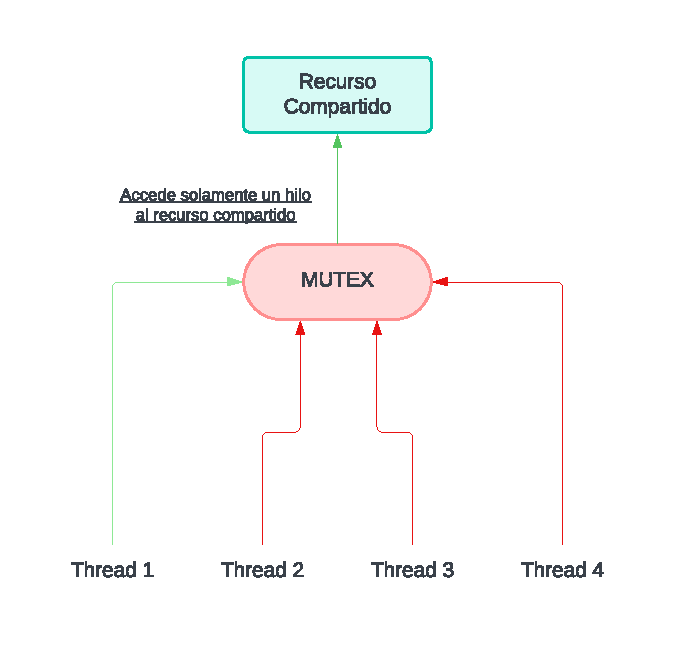
\includegraphics[width=0.35\textwidth]{src/mutex.pdf}
    \caption{Stack de un proceso multihilo}
\end{floatingfigure}
Pero si se tiene dos hilos que ejecutan el mismo código, es posible que se produzca una \myverb[blue]{condición de carrera}. Si ambos hilos leen el valor de x al mismo tiempo, ambos obtendrán el mismo valor. Luego, ambos incrementarán el valor y lo escribirán de nuevo en x. Como resultado, x solo se incrementará en 1, en lugar de 2. Para evitar este problema, se necesita una forma de asegurarse de que solo un hilo pueda ejecutar la sección crítica a la vez. Esto se puede lograr con un \textbf{lock}.

A esto lo llamamos \textbf{mutex}, que es una abreviatura de \textit{mutual exclusion}. Un mutex es una estructura de datos que se utiliza para proteger una sección crítica. Un mutex tiene dos estados: \textbf{bloqueado} y \textbf{desbloqueado}. Si un hilo intenta bloquear un mutex que ya está bloqueado, el hilo se bloqueará hasta que el mutex esté desbloqueado.

Para la utilización de locks, se pueden utilizar las siguientes funciones de la librería de POSIX, aún así es importante comprender como están implementados los locks en el sistema operativo.

\subsection{Creación de locks}

La libreria de POSIX posee funcionec que nos permiten manejar la exclusión mutua de una manera más sencilla. 

\begin{tcblisting}{colback=yellow!5, colframe=yellow!40!black, listing only, listing options={language=C, keywordstyle=\color{blue!35!white}\bfseries}}
int pthread_mutex_lock(pthread_mutex_t *mutex);
int pthread_mutex_unlock(pthread_mutex_t *mutex);
\end{tcblisting}    

Cuando se necesita proteger una sección crítica, se puede usar un \textbf{mutex} (abreviatura de \textit{mutual exclusion}). Un mutex es una estructura de datos que se utiliza para proteger una sección crítica. Un mutex tiene dos estados: \textbf{bloqueado} y \textbf{desbloqueado}. Si un hilo intenta bloquear un mutex que ya está bloqueado, el hilo se bloqueará hasta que el mutex esté desbloqueado. Veamos un ejemplo cortito:
    
\begin{tcblisting}{colback=yellow!5, colframe=yellow!40!black, listing only, listing options={language=C, keywordstyle=\color{blue!35!white}\bfseries}}
pthread_mutex_t lock;
pthread_mutex_lock(&lock);
x = x + 1; // critical section
pthread_mutex_unlock(&lock);
\end{tcblisting}  

Esto funcionaría de la siguiente manera: si ningún otro hilo tiene el bloqueo cuando se llama a \newline \texttt{pthread\_mutex\_lock()}, el hilo adquirirá el bloqueo y entrará en la sección crítica. Si otro hilo ya tiene el bloqueo, el hilo que intenta adquirirlo no regresará de la llamada hasta que lo haya conseguido.

\subsection{Inicialización de un mutex}
Para inicializar un mutex \textbf{en tiempo de ejecución}, se utiliza la función \texttt{pthread\_mutex\_init}. Esta función toma un puntero a un mutex y un puntero a una estructura de atributos de mutex. Si no se desea especificar ningún atributo, se puede pasar NULL.

\begin{tcblisting}{colback=yellow!5, colframe=yellow!40!black, listing only, listing options={language=C, keywordstyle=\color{blue!35!white}\bfseries}}
int rc = pthread_mutex_init(&lock, NULL);    
\end{tcblisting}

Otra opción es \textbf{inicializar un mutex en tiempo de compilación}. Para hacer esto, se puede declarar un mutex y asignarle el valor \texttt{PTHREAD\_MUTEX\_INITIALIZER}.

\begin{tcblisting}{colback=yellow!5, colframe=yellow!40!black, listing only, listing options={language=C, keywordstyle=\color{blue!35!white}\bfseries}}
pthread_mutex_t lock = PTHREAD_MUTEX_INITIALIZER;
\end{tcblisting}

\newpage

\subsection{Implementación de un lock}

En clase se plantea un cuadro de implementaciones del Algoritmo de la Sección Crítica:

\begin{table}[htb]
    \refstepcounter{table}\label{tab:mytab}
    \begin{tcolorbox}[tab2,tabularx*={\renewcommand{\arraystretch}{1.5}}{>{\centering\arraybackslash}Y|>{\centering\arraybackslash}Y|>{\centering\arraybackslash}Y|>{\centering\arraybackslash}Y|>{\centering\arraybackslash}Y|>{\centering\arraybackslash}Y},title={Tabla \thetable. Implementaciones del Algoritmo de la Sección Crítica},boxrule=0.8pt]
    \textbf{Solución a la CS} & \textbf{¿Exclusión Mútua?} & \textbf{¿Es justa?} & \textbf{Desempeño} & \textbf{¿MultiCore?} & \textbf{¿Requiere soporte especial del $\mu$P?}  \\\hline\hline
    \textbf{Solución homeopática}  & NO & SÍ & SÍ  & SÍ  & NO \\\hline
    \textbf{Espera infinita} & SÍ & NO & ??  & SÍ  & NO \\\hline
    \textbf{Desabilitar interrupciones} & SÍ & NO & SÍ & NO  & NO \\\hline
    \textbf{Bandera de espera} & NO & NO & Depende de la CS & SÍ & NO \\\hline
    \textbf{Spinlock Test and Set} & SÍ & NO & Depende de la CS y cores & SÍ & SÍ \\\hline
    \textbf{Spinlock Compare and Swap} & SÍ & NO & Idem pero escribe menos en memoria & SÍ & SÍ \\\hline
    \textbf{Spinlock LL SC} & SÍ & NO & Idem & SÍ & SÍ \\\hline
    \textbf{Spinlock Fetch and Add} & SÍ & SÍ & Idem & SÍ & NO \\\hline
    \textbf{Dekker ('68)} & SÍ & NO & Idem & Dual Core & NO \\\hline 
    \textbf{Peterson ('81)} & SÍ & NO & Idem & Dual Core & NO \\\hline

    \end{tcolorbox}
\end{table}

En la primera columna podemos ver las soluciones planteadas:
\begin{enumerate}
    \item \myverb[red]{Solución homeopática:} es la solución más simple, pero no es segura.
    \begin{itemize}
        \item \texttt{lock()}: skip.
        \item \texttt{unlock()}: skip.
    \end{itemize}
    \item \myverb[red]{Espera infinita}: se plantea que el lock sea un bucle infinito, esto lleva a que no haya progreso en el programa.
    \begin{itemize}
        \item \texttt{lock()}: while (1); 
        \item \texttt{unlock()}: skip;
    \end{itemize}
    \item \myverb[red]{Desabilitar interrupciones}: es una solución que nos garantiza la exclusión mútua, supongamos que dos hilos tienen una sección crítica, al entrar a la de alguno de ellos, no hay forma de que otro hilo pueda intentar entrar, ya que no se puede producir un cambio de contexto, dado que las interrupciones están desabilitadas. Pero al pensarlo en un sistema multicore \textit{no es una solución viable.} Tampoco es justa la solución, no hay nada que te asegure de que cuando un hilo quiera entrar a una zona crítica termine entrando. 
    \begin{itemize}
        \item \texttt{lock()}: CLI (disable\_interrupts());
        \item \texttt{unlock()}: STI (set\_interrupts());
    \end{itemize}
    \item \myverb[red]{Flag de espera}: es una solución que se basa en un flag que indica si un candado esta ocupado o no, acá surge el problema de que dos hilos pueden leer el flag al mismo tiempo y ambos ver que el candado está libre, por lo que ambos intentarán entrar a la sección crítica. Se produce una condición de carrera.
    \begin{itemize}
        \item \texttt{lock()}: while (lock) \{ /* busy wait */ \}; lock = 1;
        \item \texttt{unlock()}: lock = 0;
    \end{itemize}
    \item \myverb[red]{Spinlock Test and Set}: es una solución que se basa en una implementación de hardware, que nos permite hacer un test and set de un flag, nos va a dejar saber si un candado está ocupado o no. Esto nos soluciona el problema de la opción anterior, ya que el \textbf{test and set es una operación atómica.} 
    El programa impreso en hardware se vería de la siguiente manera a modo ilustrativo:
    
    \begin{tcblisting}{colback=red!5, colframe=red!40!black, listing only, listing options={language=C, keywordstyle=\color{blue!35!white}\bfseries}}
    int TestAndSet(int *old_ptr, int new) {
        int old = *old_ptr; // fetch old value at old_ptr
        *old_ptr = new; // store
        return old; // return the old value
    }
    \end{tcblisting}
    y así se implementaria el lock y unlock:
    \begin{itemize}
        \item \texttt{lock()}: while (TestAndSet(\&lock, 1)); 
        \item \texttt{unlock()}: lock = 0;
    \end{itemize}
    \textit{Al ser una operación atómica, no se puede producir una condición de carrera.}
    \item \myverb[red]{Spinlock Compare and Swap}: en vez de tener una instrucción que devuelve el valor viejo y setea el valor nuevo atomicamente, lo que hace es chequear el valor de una posición de memoria y si es igual a un valor que yo espero, \textbf{entonces atómicamente setea ese valor de memoria a un valor nuevo} y retorna el valor que se esperaba. La diferencia radica en que en la versión anterior, por mas de que el valor sea 1, siempre se setea a 1, en cambio en esta versión, si el valor es 1, no se vuelve a setear a 1.
    \begin{itemize}
        \item \texttt{lock()}: while (CompareAndSwap(\&lock, 0, 1)); 
        \item \texttt{unlock()}: lock = 0;
    \end{itemize}
    Espero un 0, si es 0, lo seteo a 1 y retorno 0, si no es 0, retorno 1. La implementación de esta función es la siguiente:
    \begin{tcblisting}{colback=red!5, colframe=red!40!black, listing only, listing options={language=C, keywordstyle=\color{blue!35!white}\bfseries}}
    int CompareAndSwap(int *ptr, int expected, int new) {
        int original = *ptr;
        if (original == expected)
            *ptr = new;
        return original;
    }
    \end{tcblisting}            
    \item \myverb[red]{Spinlock LL SC}: es una solución que se basa en una instrucción de hardware que es \textbf{Load Linked} y \textbf{Store Conditional}. La instrucción \textbf{Load Linked} carga un valor de memoria en un registro y marca la dirección de memoria como \textbf{enlazada}. La instrucción \textbf{Store Conditional} almacena un valor en una dirección de memoria enlazada si la dirección de memoria no ha sido modificada desde la última instrucción \textbf{Load Linked}. A modo ilustrativo, seria de la forma:
    \begin{tcblisting}{colback=red!5, colframe=red!40!black, listing only, listing options={language=C, keywordstyle=\color{blue!35!white}\bfseries}}
    int LoadLinked(int *ptr) {
        return *ptr;
    }

    int StoreConditional(int *ptr, int value) {
        if (no update to *ptr since LL to this addr) {
            *ptr = value;
            return 1; // success!
        else {
            return 0; // failed to update
        }
    }
    \end{tcblisting}
    \newpage
    Y en este caso el lock y unlock se verían de la siguiente manera:
    \begin{tcblisting}{colback=green!5, colframe=green!40!black, listing only, listing options={language=C, keywordstyle=\color{blue!35!white}\bfseries}}
    void lock(lock_t *lock) {
        while (1) {
            while (LoadLinked(&lock->flag) == 1)
                ; // spin until its zero
            if (StoreConditional(&lock->flag, 1) == 1)
                return; // if set-to-1 was success: done
                // otherwise: try again
        }
    }

    void unlock(lock_t *lock) {
        lock->flag = 0;
    }
    \end{tcblisting}
    Este programa es muy similar al de la bandera simple, solamente que controla el hecho de si alguien más modificó la bandera mientras yo estaba intentando modificarla.
    \item \myverb[red]{Spinlock Fetch and Add}: es una solución que se basa en una instrucción de hardware que es \textbf{Fetch and Add}. La instrucción \textbf{Fetch and Add} incrementa un valor en una dirección de memoria y devuelve el valor original. A modo ilustrativo, funciona como una ticketera, cada hilo que quiere entrar a la sección crítica, obtiene un ticket y espera a que su ticket sea el siguiente en la cola. Se vería de la siguiente manera:
    \begin{tcblisting}{colback=red!5, colframe=red!40!black, listing only, listing options={language=C, keywordstyle=\color{blue!35!white}\bfseries}}
    int FetchAndAdd(int *ptr) {
        int old = *ptr;
        *ptr = old + 1;
        return old;
    }
    \end{tcblisting}
    \begin{tcblisting}{colback=green!5, colframe=green!40!black, listing only, listing options={language=C, keywordstyle=\color{blue!35!white}\bfseries}}
    typedef struct __lock_t {
        int ticket;
        int turn;
    } lock_t;
    
    void lock_init(lock_t *lock) {
        lock->ticket = 0;
        lock->turn = 0;
    }
        
    void lock(lock_t *lock) {
        int myturn = FetchAndAdd(&lock->ticket);
        while (lock->turn != myturn)
            ; // spin
    }
        
        void unlock(lock_t *lock) {
        lock->turn = lock->turn + 1;
    }
    \end{tcblisting}            
    \item \myverb[red]{Dekker ('68)}: es una solución que se basa en dos banderas, una para cada hilo, que indican si el hilo está interesado en entrar a la sección crítica. Si ambos hilos están interesados en entrar a la sección crítica, se da prioridad a uno de los hilos. Luego el este algoritmo fue refinado por \myverb[red]{Peterson ('81)}. Usando solamente instrucciones de carga y almacenamiento, la idea es garantizar que dos hilos nunca entren en una sección crítica al mismo tiempo.
    \begin{tcblisting}{colback=green!5, colframe=green!40!black, listing only, listing options={language=C, keywordstyle=\color{blue!35!white}\bfseries}}
    int flag[2];
    int turn;
    void init() {
        // indicate you intend to hold the lock w/ flag
        flag[0] = flag[1] = 0;
        // whose turn is it? (thread 0 or 1)
        turn = 0;
    }
    void lock() {
        // self is the thread ID of caller
        flag[self] = 1;
        // make it other threads turn
        turn = 1 - self;
        while ((flag[1-self] == 1) && (turn == 1 - self))
            ; // spin-wait while its not your turn
    }
    void unlock() {
        // simply undo your intent
        flag[self] = 0;
    }
    \end{tcblisting}
\end{enumerate}

Hasta ahora, todas las soluciones implicaban que un hilo que intenta entrar a la sección crítica y no puede hacerlo, se queda esperando. Esto se llama \textbf{spinlock}, y es una forma de esperar activamente. Si bien este enfoque sirve en algunos contextos, la espera activa no es buena, si se tuviese que esperar mucho tiempo, \textit{se estaría desperdiciando recursos}. La idea es poder sacarle el mayor provecho a la CPU, y no estar esperando a que un recurso se libere. Entonces se planea otro cuadro con mas alternativas \textbf{sin tener una espera activa}:

\begin{table}[htb]
    \refstepcounter{table}\label{tab:mytab}
    \begin{tcolorbox}[tab2,tabularx*={\renewcommand{\arraystretch}{1.5}}{>{\centering\arraybackslash}Y|>{\centering\arraybackslash}Y|>{\centering\arraybackslash}Y|>{\centering\arraybackslash}Y|>{\centering\arraybackslash}Y|>{\centering\arraybackslash}Y},title={Tabla \thetable. Implementaciones del Algoritmo de la Sección Crítica \#2},boxrule=0.8pt]
    \textbf{Solución a la CS} & \textbf{¿Exclusión Mútua?} & \textbf{¿Es justa?} & \textbf{Desempeño} & \textbf{¿MultiCore?} & \textbf{¿Requiere soporte especial del $\mu$P?}  \\\hline\hline
    \textbf{Test and Set con Yield} & SÍ & NO & Está pensado para una CS grande &  SI & NO \\\hline
    \textbf{Test and Set con Yield, Park, unpark} & SÍ & NO, ya que puede haber deadlock & Está pensado para una CS grande & SI & NO \\\hline
    \end{tcolorbox}
\end{table}

\begin{enumerate}
    \item \myverb[yellow]{Yield()}: es una solución que se basa en la función \texttt{yield()}, que le dice al planificador que el hilo actual está listo para ceder el control de la CPU. Si hay otro hilo listo para ejecutarse, el planificador puede cambiar al otro hilo. Si no hay otro hilo listo para ejecutarse, el hilo actual continuará ejecutándose. Es decir si el lock no esta libre, se cede el control de la CPU a otro hilo, y se espera a que el lock se libere.
    \begin{tcblisting}{colback=green!5, colframe=green!40!black, listing only, listing options={language=C, keywordstyle=\color{blue!35!white}\bfseries}}
    void init() {
        flag = 0;
    }
            
    void lock() {
        while (TestAndSet(&flag, 1) == 1)
            yield(); // give up the CPU
    }
            
    void unlock() {
        flag = 0;
    }
    \end{tcblisting}
    \item \myverb[yellow]{Park y Unpark}: es una solución que se basa en las funciones \texttt{park()} y \texttt{unpark()}. La función \texttt{park()} le dice al planificador que el hilo actual no está listo para ejecutarse y que el planificador puede cambiar a otro hilo. La función \texttt{unpark()} le dice al planificador que el hilo actual está listo para ejecutarse. Es decir, si el lock no está libre, se llama a \texttt{park()} y se espera a que el lock se libere. Cuando el lock se libera, se llama a \texttt{unpark()} y el hilo puede entrar a la sección crítica. Acá surge una cuestión, para implementar el manejo de una sección crítica, estamos necesitando hacer de una operación que sea atómica, y acá podriamos usar un spinlock, con espera activa, la implementación de esta solución es la siguiente:
    \begin{tcblisting}{colback=green!5, colframe=green!40!black, listing only, listing options={language=C, keywordstyle=\color{blue!35!white}\bfseries}}
    typedef struct __lock_t {
        int flag;
        int guard;
        queue_t *q;
    } lock_t;

    void lock_init(lock_t *m) {
        m->flag = 0;
        m->guard = 0;
        queue_init(m->q);
    }

    void lock(lock_t *m) {
        while (TestAndSet(&m->guard, 1) == 1)
            ; //acquire guard lock by spinning
        if (m->flag == 0) {
            m->flag = 1; // lock is acquired
            m->guard = 0;
        } else {
            queue_add(m->q, gettid());
            m->guard = 0;
            park();
        }
    }
    
    void unlock(lock_t *m) {
        while (TestAndSet(&m->guard, 1) == 1)
            ; //acquire guard lock by spinning
        if (queue_empty(m->q))
            m->flag = 0; // let go of lock; no one wants it
        else
            unpark(queue_remove(m->q)); // hold lock
            // (for next thread!)
            m->guard = 0;
    }
    \end{tcblisting}
    En este caso \texttt{guard} es el lock primitivo, para implementar un lock. En la función \texttt{lock}, si el flag está en cero, se setea a 1, y se libera el guard, si no, \textbf{la región crítica estaría ocupada}, se agrega el hilo a la cola y se llama a \texttt{park()}. En la función \texttt{unlock}, si la cola está vacía, se libera el lock, si no, se llama a \texttt{unpark()} con el primero de la cola y se mantiene el lock.

    En esta implementación surge un problema, al soltar la guarda en el lock, se puede producir un \textbf{deadlock}, ya que si un hilo entra a la sección crítica y se bloquea, el siguiente hilo que quiera entrar a la sección crítica no podrá hacerlo, ya que el hilo que está bloqueado no podrá liberar el lock.
\end{enumerate}

\textit{Este problema se va a solucionar mas adelante en la sección \ref{sec:condvar}.}

\subsection{Manejo de sección crítica en Linux}

Un \textbf{futex} es una primitiva de sincronización utilizada en Linux para implementar mecanismos de bloqueo eficientes, especialmente cuando múltiples hilos comparten una misma región de memoria. Los futexes ofrecen una ventaja en términos de rendimiento al realizar la mayor parte de su operación en el espacio de usuario, recurriendo al núcleo solo cuando es estrictamente necesario, lo cual minimiza la sobrecarga de llamadas al sistema.

\begin{itemize}
    \item \myverb[blue]{futex\_wait(address,expected)}: pone al hilo en espera solo si el valor en la dirección es el mismo que el valor esperado. Esto evita que el hilo espere en vano. Si el valor no coincide, el sistema asume que no hay necesidad de esperar y regresa inmediatamente.
    \item \myverb[red]{futex\_wake(address)}: despierta a uno de los hilos que está esperando en la dirección especificada. Esto es útil para notificar a los hilos que estaban bloqueados, permitiendo que uno de ellos continúe ejecutándose.
\end{itemize}

\begin{tcblisting}{colback=yellow!5, colframe=yellow!40!black, listing only, listing options={language=C, keywordstyle=\color{blue!35!white}\bfseries}}
void mutex_lock (int *mutex) {
    int v;
    // Bit 31 estaba desactivado, obtuvimos el mutex (ruta rapida)
    if (atomic_bit_test_set (mutex, 31) == 0)
        return;
    atomic_increment (mutex);
    while (1) {
        if (atomic_bit_test_set (mutex, 31) == 0) {
            atomic_decrement (mutex);
            return;
        }
        // Debemos esperar primero para asegurarnos de que el valor del futex
        // que estamos monitoreando sea negativo (bloqueado).
        v = *mutex;
        if (v >= 0)
            continue;
        futex_wait (mutex, v);
    }
}

void mutex_unlock (int *mutex) {
    // Agregar 0x80000000 al contador resulta en 0 si y solo si no hay 
    // otros hilos interesados
    if (atomic_add_zero (mutex, 0x80000000))
        return;
    
    // Hay otros hilos esperando por este mutex,
    // despierta a uno de ellos.
    futex_wake (mutex);
}
\end{tcblisting}    
El código usa un solo entero como una estructura de datos compleja, donde \textit{el bit más alto indica si el bloqueo está retenido o no}. Si ese bit es $1$ (valor negativo en la variable), el bloqueo está activo. Cuando un hilo trata de bloquear, usa \textit{atomic\_bit\_test\_set}. Si este devuelve $0$, significa que no hay contención, y el hilo se bloquea rápidamente sin esperar.

La función \texttt{mutex\_unlock} usa el valor hexadecimal $0x80000000$ para liberar el bloqueo. Si no hay hilos en espera, simplemente libera el mutex y regresa. Si hay hilos esperando, llama a \texttt{futex\_wake} para despertar a uno de los hilos en la cola, asegurando que el bloqueo pase al siguiente en la fila.

\section{Variables de condición}\label{sec:condvar}
En ocasiones es necesario que un hilo verifique que se cumpla alguna condición antes de poder avanzar, con una variable de condición, un hilo puede bloquearse de forma atómica hasta que se cumpla una condición. La condición se prueba bajo la protección de un bloqueo de exclusión mutua (mutex).
% Para esperar que una condición se vuelva true, un hilo puede usar una condition variable. Una variable de condición es un conjunto de estructuras de datos (\textbf{cola} y \textbf{lock}) explícitos donde hilos, en algún estado de ejecución (condición) que no es deseado (como esperando en la condición, chequeando que se vuelva true); entonces algún otro hilo, cuando cambie dicho estado, puede despertar uno, o varios, de esos hilos en espera, y así permitirles que continúen (al darle una señal/signaling a la condición).
Entonces, la \myverb[blue]{variable de condición} es: algoritmos mas estructuras de datos, las estructuras de datos son \textbf{cola} y \textbf{lock}, ambos explícitos, y los algoritmos son: \textbf{inicializar}, \textbf{esperar}, \textbf{señalar}. 

\subsection{Declaración y rutinas de una variable de condición}
Para definir una variable de condición, se escribe algo como \texttt{phtread\_cond\_t c}, una variable de condición tiene dos operaciones asociadas ya mencionadas en el párrafo anterior:

\begin{itemize}
    \item \textbf{Esperar por una condición:} \myverb[blue]{wait()}: esta llamada toma un mutex como parámetro, se asume que \textit{este mutex está bloqueado cuando se llama} a \texttt{wait()}. La responsabilidad de esta función es liberar el bloqueo y poner al hilo que la llama a dormir (atómicamente); cuando el hilo se despierta (después de que otro hilo le haya enviado una señal), debe volver a adquirir el bloqueo antes de regresar al llamador.
    \item \textbf{Señalizar una condición:} \myverb[red]{signal()}: esta llamada es ejecutada cuando un hilo cambió algo que puede ser de interés para otro hilo, y despierta a un hilo que está esperando.
\end{itemize}

\begin{tcblisting}{colback=yellow!5, colframe=yellow!40!black, listing only, listing options={language=C, keywordstyle=\color{blue!35!white}\bfseries}}
pthread_cond_wait(pthread_cond_t *c, pthread_mutex_t *m);
pthread_cond_signal(pthread_cond_t *c);
\end{tcblisting}

Luego hay mas funciones que nos brinca la librería en la siguiente tabla:

\begin{table}[htb]
    \refstepcounter{table}\label{tab:mytab}
    \begin{tcolorbox}[tab2,tabularx*={\renewcommand{\arraystretch}{1.5}}{
    >{\centering\arraybackslash}Y|>{\centering\arraybackslash}Y|>{\centering\arraybackslash}Y},title={Tabla \thetable. Funciones de una variable de condición},boxrule=0.8pt]
    \textbf{Función} & \textbf{Descripción} & \textbf{Uso} \\\hline\hline
    \texttt{pthread\_cond\_init()} & Inicializa una variable de condición & \texttt{pthread\_cond\_init(\&c, NULL);} \\\hline
    \texttt{pthread\_cond\_timedwait()} & Espera por una condición con un tiempo de espera & \texttt{pthread\_cond\_timedwait(\&c, \&m, \&ts);} \\\hline
    \texttt{phtread\_cond\_reltimedwait()} & Espera por una condición con un tiempo de espera relativo & \texttt{pthread\_cond\_reltimedwait(\&c, \&m, \&ts);} \\\hline
    \texttt{pthread\_cond\_broadcast()} & Despierta a todos los hilos que están esperando & \texttt{pthread\_cond\_broadcast(\&c);} \\\hline
    \texttt{pthread\_cond\_destroy()} & Destruye una variable de condición & \texttt{pthread\_cond\_destroy(\&c);} \\\hline
    \end{tcolorbox}
\end{table}
\newpage
\subsection{Ejemplo de uso de una variable de condición}

Tenemos el problema planteado al inicio de la sección, se hace esperar al padre hasta que el hijo termine de ejecutarse. Para esto se plantea el siguiente código:

\begin{tcblisting}{colback=yellow!5, colframe=yellow!40!black, listing only, listing options={language=C, keywordstyle=\color{blue!35!white}\bfseries}}
volatile int done = 0;

void *child(void *arg) {
    printf("child\n");
    done = 1;
    return NULL;
}

int main(int argc, char *argv[]) {
    printf("parent: begin\n");
    pthread_t c;
    Pthread_create(&c, NULL, child, NULL); // child
    while (done == 0)
        ; // spin
    printf("parent: end\n");
    return 0;
}
\end{tcblisting}    

En este código se plantea que el padre espere a que el hijo termine de ejecutarse, pero esto no es una buena práctica, ya que se está desperdiciando recursos, se tiene una espera activa. 

Ahora la idea es considerar dos casos posibles:
\begin{enumerate}
    \item El padre crea el hilo hijo pero continúa ejecutándose él mismo y, por lo tanto, llama inmediatamente a \textbf{thr\_join()} para esperar que el hilo hijo termine. En este caso, adquirirá el bloqueo, verificará si el hijo ha terminado y se pondrá a dormir llamando a \texttt{wait()} (liberando así el bloqueo). Eventualmente, el hilo hijo se ejecutará, imprimirá el mensaje "child" y llamará a \texttt{thr\_exit()} para despertar al hilo padre; este código simplemente toma el bloqueo, establece la variable de estado done, y envía una señal al hilo padre para despertarlo. Finalmente, el padre se ejecutará (regresando de wait() con el bloqueo adquirido), liberará el bloqueo y por último imprimirá el mensaje final "parent: end".
    \item En el segundo caso, el hilo hijo se ejecuta inmediatamente después de ser creado, \textit{establece done a 1}, llama a signal para despertar a un hilo en espera (pero no hay ninguno, así que simplemente retorna) y termina. Luego, el hilo padre se ejecuta, llama a \texttt{thr\_join()}, ve que done es 1, y por lo tanto no espera y retorna.
\end{enumerate}

Conclusión, padre e hijo cumplen las siguientes funciones:

\begin{itemize}
    \item \textbf{Padre:}
    \begin{enumerate}
        \item Crea el hilo hijo y continúa ejecutándose.
        \item Llama a \texttt{thr\_join()} para esperar a que el hilo hijo termine:
        \begin{itemize}
            \item Adquiero el lock.
            \item Verifico si el hijo ha terminado.
            \item Se pone en espera llamando a \texttt{wait()}.
            \item Libera el lock.
        \end{itemize}
    \end{enumerate}
    \item \textbf{Hijo:}
    \begin{enumerate}
        \item Imprime el mensaje "child".
        \item Llama a \texttt{thr\_exit()} para despertar al hilo padre:
        \begin{itemize}
            \item Adquiere el lock.
            \item Fija la variable de estado \texttt{done}.
            \item Señaliza al hilo padre llamando a \texttt{signal()}.
        \end{itemize}
    \end{enumerate}
\end{itemize}

\newpage
\begin{tcblisting}{colback=yellow!5, colframe=yellow!40!black, listing only, listing options={language=C, keywordstyle=\color{blue!35!white}\bfseries}}
int done = 0;
pthread_mutex_t m = PTHREAD_MUTEX_INITIALIZER;
pthread_cond_t c = PTHREAD_COND_INITIALIZER;
    
void thr_exit() {
    Pthread_mutex_lock(&m);
    done = 1;
    Pthread_cond_signal(&c);
    Pthread_mutex_unlock(&m);
}
    
void *child(void *arg) {
    printf("child\n");
    thr_exit();
    return NULL;
}

void thr_join() {
    Pthread_mutex_lock(&m);
    while (done == 0)
        Pthread_cond_wait(&c, &m);
    Pthread_mutex_unlock(&m);
}

int main(int argc, char *argv[]) {
    printf("parent: begin\n");
    pthread_t p;
    Pthread_create(&p, NULL, child, NULL);
    thr_join();
    printf("parent: end\n");
    return 0;
}
\end{tcblisting}    

\subsubsection{Importancia de variable de estado}
Ahora bien, que pasaría si quisiéramos implementar las funciones de \texttt{thr\_join()} y \texttt{thr\_exit()} \textit{sin utilizar una variable de estado done}. Que nos permitía saber si el hilo hijo había terminado o no. Para esto se plantea el siguiente código:

\begin{tcblisting}{colback=yellow!5, colframe=yellow!40!black, listing only, listing options={language=C, keywordstyle=\color{blue!35!white}\bfseries}}
void thr_exit() {
    Pthread_mutex_lock(&m);
    Pthread_cond_signal(&c);
    Pthread_mutex_unlock(&m);
}

void thr_join() {
    Pthread_mutex_lock(&m);
    Pthread_cond_wait(&c, &m);
    Pthread_mutex_unlock(&m);
}
\end{tcblisting}

Pero en este caso, que pasaría si el padre crea un hijo hijo, y este se ejecuta primero, este va a mandar una señal al padre, pero el padre no está esperando, entonces el hilo hijo se va a quedar esperando a que el padre lo despierte. Luego el padre cuando llame a wait quedará bloqueado eternamente.

\subsubsection{Importancia del mutex}

Si no tuviesemos un mutex, el código sería el siguiente:

\begin{tcblisting}{colback=yellow!5, colframe=yellow!40!black, listing only, listing options={language=C, keywordstyle=\color{blue!35!white}\bfseries}}
void thr_exit() {
    done = 1;
    Pthread_cond_signal(&c);
}
        
void thr_join() {
    if (done == 0)
        Pthread_cond_wait(&c);
}
\end{tcblisting}

Acá trivialmente, se puede ver que se va a producir una condición de carrera, el padre puede ser interrumpido antes de llamar a wait, el cambio de contexto se produce hacia el hijo, este finaliza y llama a signal sin haber nadie esperando, y luego el padre corre denuevo y queda bloqueado indefinidamente.


\subsection{Problema del productor-consumidor}

Este es un problema clásico de concurrencia, se plantea de la siguiente manera:

\begin{tcolorbox}
    \textbf{Problema del productor-consumidor:} 
    \tcblower
    Imaginemos uno o más hilos productores y uno o más hilos consumidores. Los productores general elementos de datos y los colocan en un buffer; los consumidores obtienen dichos elementos y los consumen de alguna forma. Como este buffer es un recurso compartido se necesita alguna clase de sincronización para acceder a este, para evitar una condición de carrera.
    \begin{center}
        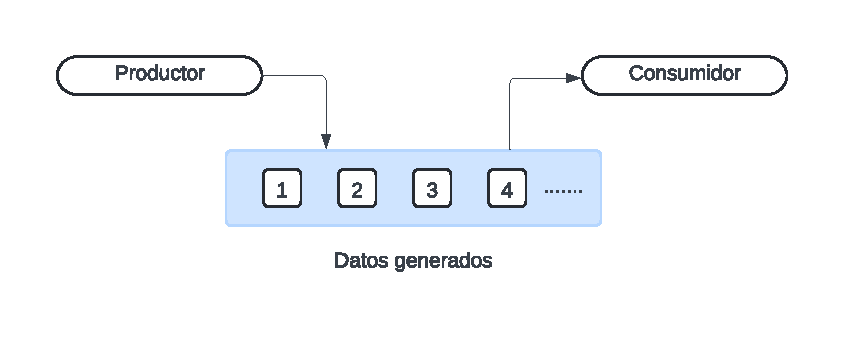
\includegraphics[scale=0.5]{src/prodconsu.pdf}    
    \end{center}
\end{tcolorbox}

Para resolver este problema, se plantea la siguiente solución, el buffer en este caso es simplemente un entero, es decir puedo almacenar un solo ítem, también tengo un contador de items. Las funcion \texttt{put()} va a ser llamada por el productor para poner un valor en el ítem y luego \texttt{get()} va a ser llamada por el consumidor para obtener el valor del ítem.

\begin{tcblisting}{colback=yellow!5, colframe=yellow!40!black, listing only, listing options={language=C, keywordstyle=\color{blue!35!white}\bfseries}}
int buffer;
int count = 0; // initially, empty
    
void put(int value) {
    assert(count == 0);
    count = 1;
    buffer = value;
}
    
int get() {
    assert(count == 1);
    count = 0;
    return buffer;
}
\end{tcblisting}

Lo que hay que hacer es encontrar la forma de sincronizar, para ello planteamos lo siguiente:

\begin{enumerate}
    \item Implementación con variables de condición: 
    \begin{itemize}
        \item \textbf{Productor:} cuando vamos a producir, vamos a llamar a un mutex, con la variable contador vamos a verificar si está en 1, si es así, significa que el buffer esta lleno, entonces vamos a esperar a que se vacíe, y luego vamos a poner el valor en el buffer. Cuando vamos a consumir, vamos a verificar si el contador es 0, si es así, significa que el buffer está vacío, entonces se manda a dormir. Si no se cumple, quiere decir que si puede producir, produce un item, y manda una señal a un proceso que puede estar dormido esperando a que se produzca un item. 
        \item \textbf{Consumidor:} se llama a un mutex para acceder a la región crítica, preguntamos si el consumidor puede consumir (variable contador en 1), si no puede consumir se va a dormir, si puede consumir, consume el item, y manda una señal al productor para que produzca un item y por último se libera el mutex.
    \end{itemize}
    \begin{tcblisting}{colback=yellow!5, colframe=yellow!40!black, listing only, listing options={language=C, keywordstyle=\color{blue!35!white}\bfseries}}
        int loops; // must initialize somewhere...
        cond_t cond;
        mutex_t mutex;
        
        void *producer(void *arg) {
            int i;
            for (i = 0; i < loops; i++) {
                Pthread_mutex_lock(&mutex); // p1
                if (count == 1) // p2
                    Pthread_cond_wait(&cond, &mutex); // p3
                put(i); // p4
                Pthread_cond_signal(&cond); // p5
                Pthread_mutex_unlock(&mutex); // p6
            }
        }
        
        void *consumer(void *arg) {
            int i;
            for (i = 0; i < loops; i++) {
                Pthread_mutex_lock(&mutex); // c1
                if (count == 0) // c2
                    Pthread_cond_wait(&cond, &mutex); // c3
                int tmp = get(); // c4
                Pthread_cond_signal(&cond); // c5
                Pthread_mutex_unlock(&mutex); // c6
                printf("%d\n", tmp);
            }
        }
        \end{tcblisting}
        Este código va a funcionar siempre y cuando tengamos un consumidor y un productor, si tuviésemos más de un consumidor o productor, se podría producir un \textbf{deadlock}.
        \newpage
        \item Implementación con variables de condición y un while: en esta versión el no usar un if, sino un while, se evita el problema anterior, ya que si un hilo se despierta y no puede consumir, se vuelve a dormir. Siempre que haya variables de condición es recomendable usar un while.
        \begin{tcblisting}{colback=yellow!5, colframe=yellow!40!black, listing only, listing options={language=C, keywordstyle=\color{blue!35!white}\bfseries}}
        int loops;
        cond_t cond;
        mutex_t mutex;
            
        void *producer(void *arg) {
            int i;
            for (i = 0; i < loops; i++) {
                Pthread_mutex_lock(&mutex); // p1
                while (count == 1) // p2
                    Pthread_cond_wait(&cond, &mutex); // p3
                put(i); // p4
                Pthread_cond_signal(&cond); // p5
                Pthread_mutex_unlock(&mutex); // p6
            }
        }
            
        void *consumer(void *arg) {
            int i;
            for (i = 0; i < loops; i++) {
                Pthread_mutex_lock(&mutex); // c1
                while (count == 0) // c2
                    Pthread_cond_wait(&cond, &mutex); // c3
                int tmp = get(); // c4
                Pthread_cond_signal(&cond); // c5
                Pthread_mutex_unlock(&mutex); // c6
                printf("%d\n", tmp);
            }
        }
        \end{tcblisting}
        Todavía hay un problema, puede pasar que dos consumidores quieran consumir, el buffer está vacío, se duermen, luego un productor llena el buffer, después, como está lleno el buffer duerme a la vez que da la señal que despierta algún consumidor. Digamos consumidor 1, este consume el buffer, da la señal de que está vacío y duerme, pero que hilo se despierta (estan durmiendo productor 1 y consumidor 2 en la mismo condición) si se despierta productor 1 funciona, pero si despierta consumidor 2 se encontraría el buffer vació y dormiría. Ahora todos duermen indefinidamente. El error es que las señales deberían ser más directas, un consumidor no debería poder despertar a otros consumidores y viceversa. Este problema se soluciona de una manera muy sencilla, \textbf{usando dos variables de condición}, una que me indique si el buffer esta lleno y otra que me indique si esta vacío.

        \newpage
        \item Implementación con dos variables de condición: en este caso se plantea la solución al problema anterior, se plantea una variable de condición para saber si el buffer está lleno y otra para saber si está vacío.
        \begin{itemize}
            \item Productor se va a dormir usando la variable \texttt{empty}, y señaliza \texttt{fill}.
            \item Consumidor se va a dormir usando la variable \texttt{fill}, y señaliza \texttt{empty}.
        \end{itemize}
        \begin{tcblisting}{colback=yellow!5, colframe=yellow!40!black, listing only, listing options={language=C, keywordstyle=\color{blue!35!white}\bfseries}}
        cond_t empty, fill;
        mutex_t mutex;
            
        void *producer(void *arg) {
            int i;
            for (i = 0; i < loops; i++) {
                Pthread_mutex_lock(&mutex);
                while (count == 1)
                    Pthread_cond_wait(&empty, &mutex);
                put(i);
                Pthread_cond_signal(&fill);
                Pthread_mutex_unlock(&mutex);
            }
        }
            
        void *consumer(void *arg) {
            int i;
            for (i = 0; i < loops; i++) {
                Pthread_mutex_lock(&mutex);
                while (count == 0)
                  Pthread_cond_wait(&fill, &mutex);
                int tmp = get();
                Pthread_cond_signal(&empty);
                Pthread_mutex_unlock(&mutex);
                printf("%d\n", tmp);
            }
        }
        \end{tcblisting}    
        De esta manera nos aseguramos de que el productor solo despierte a los consumidores y viceversa.        
\end{enumerate}

Luego la solución se puede extender tomando un buffer que no sea simplemente un entero, sino un arreglo de enteros.

\section{Semáforos}

Un \textbf{semáforo} es una estructura de sincronización en programación concurrente que gestiona el acceso a recursos compartidos. Consiste en un valor entero que se incrementa o decrementa mediante las funciones \texttt{sem\_wait()} (decremento) y \texttt{sem\_post()} (incremento) para coordinar la ejecución entre múltiples hilos o procesos.

\begin{itemize}
    \item \texttt{sem\_wait()}: Decrementa el valor del semáforo. Si el valor es menor que cero, el hilo que llama se bloquea hasta que otro hilo ejecute \texttt{sem\_post()}.
    \item \texttt{sem\_post()}: Incrementa el valor del semáforo. Si algún hilo estaba bloqueado esperando el semáforo, \texttt{sem\_post()} despierta uno de estos hilos.
\end{itemize}

\subsection{Semáforos binarios}

Los semáforos binarios son semáforos cuyo valor solo puede ser 0 o 1, y se usan para implementar locks, ya que permiten que un solo hilo acceda a una sección crítica al mismo tiempo. Son inicializados con el valor 1, representando la disponibilidad del recurso.

\begin{tcblisting}{colback=yellow!5, colframe=yellow!40!black, listing only, listing options={language=C, keywordstyle=\color{blue!35!white}\bfseries}}
sem_t m;
sem_init(&m, 0, X); // init to X; 
    
sem_wait(&m);
// critical section here
sem_post(&m);
\end{tcblisting}

Simplemente rodeamos la sección crítica de interés con un par de \texttt{sem\_wait()}/\texttt{sem\_post()}. Para que esto funcione es crítico que el valor inicial sea 1. Si viene más de un hilo, el primero dejará el valor en 0 luego de entrar en la zona crítica, el siguiente hilo que quiera entrar será suspendido/dormirá y dejará el sem en -1, termina el hilo 1, deja el sem en 0, el hilo 2 despierta, adquiere el lock, entra en la sección crítica y para cuando termina el sem queda de nuevo en 1. Como los locks solo tienen dos estados.

\subsection{Semáforos para ordenar la ejecución de hilos}

Además de controlar el acceso a recursos, los semáforos se usan para ordenar eventos, permitiendo que un hilo espere hasta que otro hilo complete una tarea específica. Esto se logra inicializando el semáforo en 0 y usando sem\_wait() para que un hilo espere mientras otro hilo lo libera con sem\_post().

\begin{tcblisting}{colback=yellow!5, colframe=yellow!40!black, listing only, listing options={language=C, keywordstyle=\color{blue!35!white}\bfseries}}
sem_t s;
    
void *child(void *arg) {
    printf("child\n");
    sem_post(&s); // signal here: child is done
    return NULL;
}

int main(int argc, char *argv[]) {
    sem_init(&s, 0, X); // what should X be?
    printf("parent: begin\n");
    pthread_t c;
    Pthread_create(&c, NULL, child, NULL);
    sem_wait(&s); // wait here for child
    printf("parent: end\n");
    return 0;
}
\end{tcblisting}

\newpage
\subsection{Solución al problema del productor-consumidor con semáforos - Buffer complejo}

Para este problema se plantea la siguiente estructura de datos:

\begin{tcblisting}{colback=yellow!5, colframe=yellow!40!black, listing only, listing options={language=C, keywordstyle=\color{blue!35!white}\bfseries}}
typedef struct {
    char buf[BSIZE];
    sem_t occupied;
    sem_t empty;
    int nextin;
    int nextout;
    sem_t pmut;
    sem_t cmut;
} buffer_t;

buffer_t buffer;

sem_init(&buffer.occupied, 0, 0);
sem_init(&buffer.empty,0, BSIZE);
sem_init(&buffer.pmut, 0, 1);
sem_init(&buffer.cmut, 0, 1);
buffer.nextin = buffer.nextout = 0;
\end{tcblisting}

Dos semáforos representan la cantidad de buffers llenos y vacíos y garantizan que los productores esperen hasta que haya buffers vacíos y que los consumidores esperen hasta que haya buffers llenos.

Luego, otro par de semáforos (binarios) desempeñan la misma función que los mutex, controlando el acceso al búfer cuando hay varios productores y varias ranuras de búfer vacías, y cuando hay varios consumidores y varias ranuras de búfer llenas. Los mutex funcionarían mejor en este caso, pero no proporcionarían un ejemplo tan bueno del uso de semáforos.

\begin{tcblisting}{colback=yellow!5, colframe=yellow!40!black,title= El productor, listing only, listing options={language=C, keywordstyle=\color{blue!35!white}\bfseries}}
void producer(buffer_t *b, char item) {
    sem_wait(&b->empty);
    sem_wait(&b->pmut);
    b->buf[b->nextin] = item;
    b->nextin++;
    b->nextin %= BSIZE;
    sem_post(&b->pmut);
    sem_post(&b->occupied);
}
\end{tcblisting}

\begin{tcblisting}{colback=yellow!5, colframe=yellow!40!black,title= El consumidor, listing only, listing options={language=C, keywordstyle=\color{blue!35!white}\bfseries}}
char consumer(buffer_t *b) {
    char item;
    sem_wait(&b->occupied);
    sem_wait(&b->cmut);
    item = b->buf[b->nextout];
    b->nextout++;
    b->nextout %= BSIZE;
    sem_post(&b->cmut);
    sem_post(&b->empty);
    return(item);
}
\end{tcblisting}

\subsection{Implementación de semáforos}

Ahora se usarán nuestras primitivas de sincronización de bajo nivel, como bloqueos (locks) y variables de condición, para construir una versión de semáforos.

\begin{tcblisting}{colback=yellow!5, colframe=yellow!40!black, listing only, listing options={language=C, keywordstyle=\color{blue!35!white}\bfseries}}
typedef struct __Zem_t {
    int value;
    pthread_cond_t cond;
    pthread_mutex_t lock;
} Zem_t;

// solo un hilo puede llamar a esto
void Zem_init(Zem_t *s, int value) {
    s->value = value;
    Cond_init(&s->cond);
    Mutex_init(&s->lock);
}
\end{tcblisting}  

\begin{tcblisting}{colback=yellow!5, colframe=yellow!40!black, listing only, listing options={language=C, keywordstyle=\color{blue!35!white}\bfseries}}
void Zem_wait(Zem_t *s) {
    Mutex_lock(&s->lock);
    while (s->value <= 0)
        Cond_wait(&s->cond, &s->lock);
    s->value--;
    Mutex_unlock(&s->lock);
}

void Zem_post(Zem_t *s) {
    Mutex_lock(&s->lock);
    s->value++;
    Cond_signal(&s->cond);
    Mutex_unlock(&s->lock);
}
\end{tcblisting}    

\section{Problemas típicos de concurrencia}

\begin{itemize}
    \item \myverb[blue]{Non-Deadlock Bugs}: este tipo de errores son los más comunes en concurrencia:
    \begin{enumerate}
        \item \textbf{Errores de Violación de Atomicidad:} este problema surge cuando la señalización entre múltiples accesos a memoria es violada, este error se soluciona \textit{agregando bloqueos} alrededor de las zonas conflictivas.
        \item \textbf{Errores de Violación de Orden:} este problema hace referencia a cuando el orden entre los accesos a la memoria se invierten, la solución a este error es simple, \textit{imponer un orden} con el uso de variables de condición.
    \end{enumerate}
    \item \myverb[red]{Deadlock Bugs}: este tipo de errores son los más difíciles de solucionar, ya que se necesita un análisis más profundo para encontrar la raíz del problema. Ocurre por ejemplo cuando un hilo tiene un bloqueo (L1) y está esperando otro (L2); desafortunadamente, el hilo que tiene el bloqueo L2 está esperando a que se libere L1.
    \begin{tcblisting}{colback=red!5, colframe=red!40!black, listing only, listing options={language=C, keywordstyle=\color{blue!35!white}\bfseries}}
    // Hilo 1:                // Hilo 2:
    pthread_mutex_lock(L1);   pthread_mutex_lock(L2);
    pthread_mutex_lock(L2);   pthread_mutex_lock(L1);
    \end{tcblisting}        
    Si este código se ejecuta, el interbloqueo no necesariamente ocurre; más bien, puede ocurrir si, por ejemplo, el Hilo 1 obtiene el bloqueo L1 y luego ocurre un cambio de contexto al Hilo 2. En ese momento, el Hilo 2 obtiene L2 e intenta adquirir L1. Visualmente se puede ver como un ciclo en un grafo dirigido:
    \begin{center}
        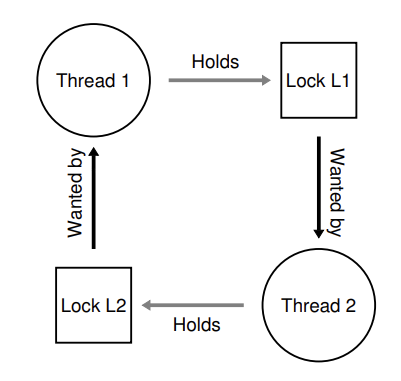
\includegraphics[scale=0.7]{src/deadlock.png}
        \begin{tcolorbox}[colback=red!5, colframe=red!40!black]
            \textbf{Deadlock:} Cada hilo está esperando al otro y ninguno puede continuar.
        \end{tcolorbox}
    \end{center}
    Para que se produzca un interbloqueo, se deben cumplir cuatro condiciones:
    \begin{itemize}
        \item \textbf{Exclusión mutua}: Los hilos reclaman control exclusivo sobre los recursos que requieren (por ejemplo, un hilo adquiere un bloqueo).
        \item \textbf{Espera y retención}: Los hilos retienen recursos asignados a ellos (por ejemplo, bloqueos que ya han adquirido) mientras esperan recursos adicionales (por ejemplo, bloqueos que desean adquirir).
        \item \textbf{Sin expropiación}: Los recursos (por ejemplo, bloqueos) no pueden ser forzados a retirarse de los hilos que los están reteniendo.
        \item \textbf{Espera circular}: Existe una cadena circular de hilos tal que cada hilo posee uno o más recursos (por ejemplo, bloqueos) que están siendo solicitados por el siguiente hilo en la cadena.
    \end{itemize}
    Algunas estrategias para evitar que se cumplan estas condiciones son:
    \begin{itemize}
        \item Evitar \myverb[blue]{exclusión mutua}: esta técnica es difícil de implementar, sería evitar del todo la necesidad de exclusión mutua mediante estructuras de datos que no requieran locks usando instrucciones de hardware.
        \item Evitar \myverb[blue]{espera y retención}: este problema se puede solucionar adquiriendo todos los bloqueos necesarios al mismo tiempo, si no se pueden adquirir todos los bloqueos, se liberan los que se han adquirido. Esto tiene algunos problemas, la encapsulación nos juega en contra, se necesitaria saber de antemano qué lock requiere el hilo para obtenerlos de antemano. Esto también disminuye la concurrencia, ya que los locks son controlados de antemano en vez que solo cuando son necesarios para el hilo.
        \item Evitar \myverb[blue]{sin expropiación}: esta técnica se basa en manejar el caso en que un hilo no puede obtener un lock, hay librerias que nos dan rutinas para evitar que un hilo se quede esperando indefinidamente, como \texttt{pthread\_mutex\_trylock()}, que intenta adquirir un lock, si no puede, retorna inmediatamente. Pero esto puede llevar a nuevos problemas, puede evitarse el deadlock por ejemplo si dos hilos intentan y ninguno puede obtenerlo, pero el programa no va a progresar. Y al solucionar este error poniendo un "retraso" en la espera, se puede caer en un problema de encapsulación.
        \item Evitar \myverb[green]{espera circular}: esta técnica se basa en imponer un orden en la adquisición de los locks, por ejemplo, si un hilo necesita adquirir dos locks, se le puede imponer que adquiera el lock 1 antes que el lock 2, de esta manera se evita que se produzca un ciclo.
    \end{itemize}
    También se puede \textbf{evitar el interbloqueo desde el planificador}, al conocer los locks globales que se están utilizando, el planificador puede evitar que se produzca un interbloqueo ejecutando los hilos de manera que no se produzca un ciclo, pero esto va a disminuir la concurrencia. No es una solución muy buena.

    La última estrategia para evitar el interbloqueo es \textbf{la detección y recuperación del interbloqueo}, en este caso se detecta el interbloqueo y se recupera de él, por ejemplo, si se detecta un interbloqueo, se puede liberar todos los locks y volver a intentar adquirirlos. Es una solución muy usada en bases de datos, pero no es muy buena, ya que se pierde el progreso del programa.
\end{itemize}

\newpage
\chapter{Persistencia y sistemas de archivos}

\begin{tcolorbox}[colback=black!5!white,colframe=black!75!black]
    Capítulos del OSTEP: 36, 37, 38, 39, 40, 41, 42, 44
\end{tcolorbox}

\section{Dispositivos de entrada/salida}
\begin{floatingfigure}[r]{0.5\textwidth}
    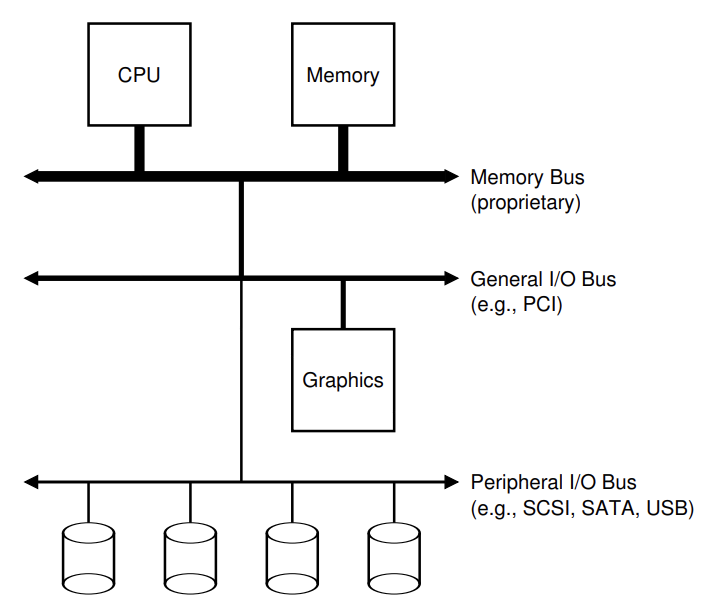
\includegraphics[width=0.5\textwidth]{src/io.png}
    \caption{Arquitectura de un sistema de computación}
\end{floatingfigure}

La imagen muestra una sola CPU conectada a la memoria principal del sistema a través de algún tipo de bus de memoria o interconector. Algunos dispositivos están conectados al sistema a través de un Bus de I/O, que en muchos sistemas modernos sería el PCI (o uno de sus muchos derivados). Los gráficos (placa gráfica) y algunos otros dispositivos de I/O de mayor rendimiento se pueden encontrar aquí. Finalmente, aún más abajo hay uno o más de lo que llamamos bus periférico, tal como SCSI, SATA, o USB. Estos conectan dispositivos lentos al sistema, incluidos discos, mouse’s, y teclados. 

\colorbox{yellow!20}{Mientras más rápido es un bus, más corto} debe ser; por lo tanto, un bus de memoria de alto rendimiento no tiene mucho espacio para conectar dispositivos. Además, diseñar un bus de alto rendimiento es bastante costoso. Por lo tanto, los/as diseñadores/as de sistemas han adoptado este enfoque jerárquico, donde los \colorbox{yellow!20}{componentes que exigen un alto}\newline \colorbox{yellow!20}{rendimiento} (como la tarjeta gráfica) \colorbox{yellow!20}{están más cerca} \colorbox{yellow!20}{de la CPU}. Los \colorbox{yellow!20}{componentes de menor rendimiento están más lejos}. Los beneficios de colocar discos y otros dispositivos lentos en un bus periférico son múltiples; en particular, podés colocar una gran cantidad de dispositivos en él. Por lo tanto sería mas fructífero ver y analizar como funcionan las arquitecturas mordernas. 

\begin{floatingfigure}[r]{0.5\textwidth}
    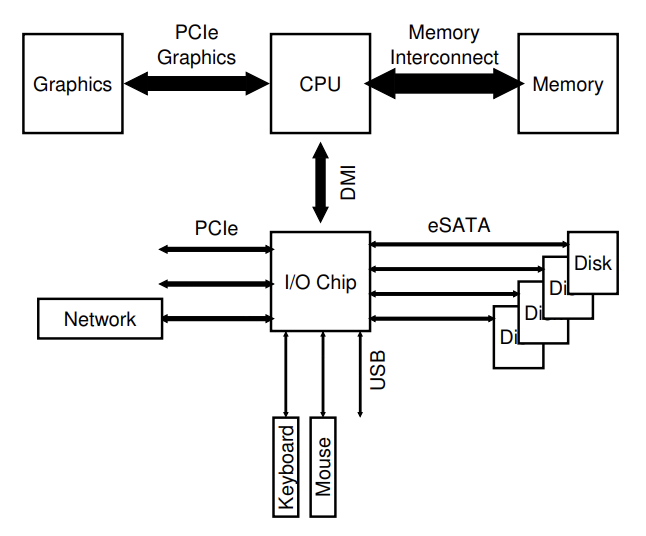
\includegraphics[width=0.5\textwidth]{src/iomoderno.png}
    \caption{Arquitectura moderna}
\end{floatingfigure}

La CPU \colorbox{yellow!20}{se conecta a un chip de I/O} a través del DMI (Direct Media Interface), y \textit{el resto de los dispositivos se conectan a este chip} a través de varias interconectores diferentes. 
\textbf{A la derecha}, uno o más \colorbox{yellow!20}{discos duros} se conectan al sistema a través de la interfaz eSATA (external data). 

\textbf{Debajo del chip} de I/O hay varias \colorbox{yellow!20}{conexiones USB} (Universal Serial Bus), que en esta ilustración permiten conectar un teclado y un mouse a la computadora. 

Finalmente, a la izquierda, se pueden conectar otros \colorbox{yellow!20}{dispositivos de mayor rendimiento} al sistema a través de PCIe (Peripheral Component Interconnect Express, en español Interconexión rápida de componentes periféricos). 

En este diagrama, se adjunta una interfaz de red al sistema; los dispositivos de almacenamiento de mayor rendimiento (como NVMe dispositivos de almacenamiento persistentes) a menudo están conectados aquí.

\newpage
\subsection{Dispositivo canónico}

Se tiene un dispositivo canónico que tiene dos componentes importantes. El primero es la \colorbox{yellow!20}{interfaz de hardware} que se presenta al resto del sistema. Al igual que una pieza de software, el hardware también debe presentar algún tipo de interfaz que permita al software del sistema controlar su funcionamiento. Por lo tanto, todos los dispositivos tienen una interfaz y un protocolo específico para una interacción típica.

\begin{floatingfigure}[r]{0.5\textwidth}
    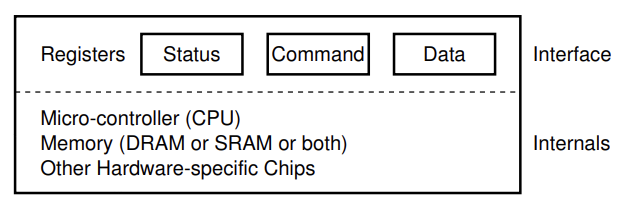
\includegraphics[width=0.5\textwidth]{src/candevice.png}
    \caption{Estructura de un dispositivo canónico}
\end{floatingfigure}

La segunda parte de cualquier dispositivo es su \colorbox{yellow!20}{estructura interna}. Esta parte del dispositivo es específica de la implementación y es responsable de implementar la abstracción que el dispositivo presenta al sistema. Los dispositivos muy simples tendrán uno o varios chips de hardware para implementar su funcionalidad; los dispositivos más complejos incluirán una CPU simple, algo de memoria de propósito general y otros chips específicos del dispositivo para hacer su trabajo.

La interfaz del dispositivo (simplificada) se compone de tres registros: un \textbf{registro de estado}, que se puede leer para ver el estado actual del dispositivo; un \textbf{registro de comando}, para decirle al dispositivo que realice una determinada tarea; y un \textbf{registro de datos}, para pasar datos al dispositivo u obtener datos del dispositivo. Con esto el sistema operativo puede \colorbox{yellow!20}{controlar el dispositivo}.

\begin{tcblisting}{colback=brown!5, colframe=brown!40!black, listing only, listing options={language=C, keywordstyle=\color{blue!35!white}\bfseries}}
While (STATUS == BUSY)
; // wait until device is not busy
Write data to DATA register
Write command to COMMAND register
(starts the device and executes the command)
While (STATUS == BUSY)
; // wait until device is done with your request
\end{tcblisting}

Este protocolo de comunicación tiene cuatro pasos:

\begin{enumerate}
    \item \myverb[blue]{Polling:} el SO espera hasta que el dispositivo esté listo para recibir un comando leyendo repetidamente el registro de estado.
    \item El SO envía algunos datos al registro de datos Cuando la CPU principal está involucrada con el movimiento de datos (como en este protocolo de ejemplo), nos referimos a ella como \myverb[blue]{I/O programado (PIO)} o entrada/salida programada.
    \item El SO \myverb[blue]{escribe} un comando en el registro de comandos; al hacerlo, implícitamente le hace saber al dispositivo que los datos están presentes y que debe comenzar a trabajar en el comando.
    \item Finalmente, el SO \myverb[blue]{espera a que el dispositivo termine} haciendo polling en un bucle, esperando para ver si está terminado.
\end{enumerate}

\subsection{Solución a la sobrecarga del polling}

En lugar de hacer polling al dispositivo repetidamente, el SO puede emitir una solicitud, poner el proceso de llamada en suspensión y cambiar de contexto a otra tarea. Basicamente los dos escenarios son:

\begin{figure}[h]
    \centering
    \begin{subfigure}[b]{0.47\textwidth}
        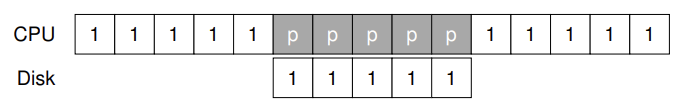
\includegraphics[width=\textwidth]{src/polling.png}
        \caption{Polling}
    \end{subfigure}
    \begin{subfigure}[b]{0.47\textwidth}
        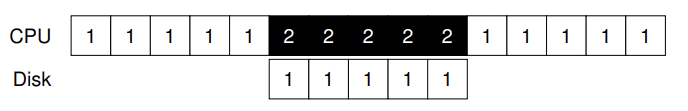
\includegraphics[width=\textwidth]{src/nopolling.png}
        \caption{Interrupción}
    \end{subfigure}
\end{figure}

Aunque las interrupciones permiten la superposición de cómputo e I/O, \textit{solo tienen sentido para dispositivos lentos}. De lo contrario, el \colorbox{yellow!20}{costo del manejo de la interrupción y el cambio de contexto} pueden superar los beneficios que brindan las interrupciones. También hay casos en los que una \colorbox{yellow!20}{avalancha de interrupciones} puede sobrecargar un sistema y provocar un livelock, en tales casos, el polling proporciona más control al SO en su planificación y, por lo tanto, vuelve a ser útil.

\subsection{Movimiento de datos más eficiente con DMA}

En particular, cuando se usa la entrada/salida programada (PIO) para transferir una gran cantidad de datos a un dispositivo, la CPU vuelve a estar sobrecargada con una tarea bastante trivial y, por lo tanto, pierde mucho tiempo y esfuerzo que podría dedicar a ejecutar otros procesos. 

Con PIO, la CPU pasa demasiado tiempo moviendo datos de y desde dispositivos a mano. ¿Cómo podemos descargar este trabajo y así permitir que la CPU se utilice de manera más efectiva?

La solución a este problema es algo a lo que nos referimos como \textbf{Acceso directo a memoria} (DMA, las siglas en inglés de Direct Memory Access). Un motor DMA es esencialmente un dispositivo muy específico dentro de un sistema que puede realizar transferencias entre dispositivos y la memoria principal sin mucha intervención de la CPU.
El DMA funciona de la siguiente manera. Para transferir datos al dispositivo, el SO programaría el motor DMA indicándole \colorbox{yellow!20}{dónde} se encuentran los datos en la memoria, \colorbox{yellow!20}{cuántos} datos copiar y \colorbox{yellow!20}{a qué dispositivo enviarlos}. A ese punto, el SO terminó con la transferencia y \colorbox{yellow!20}{puede continuar con otros trabajos}. \textit{Cuando el DMA finaliza, el controlador DMA genera una interrupción}. Ahora se ilustran los escenarios con y sin DMA.

\begin{figure}[h]
    \centering
    \begin{subfigure}[b]{0.47\textwidth}
        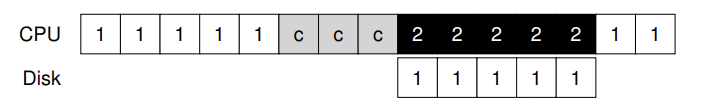
\includegraphics[width=\textwidth]{src/nodma.png}
        \caption{Sin DMA}
    \end{subfigure}
    \begin{subfigure}[b]{0.47\textwidth}
        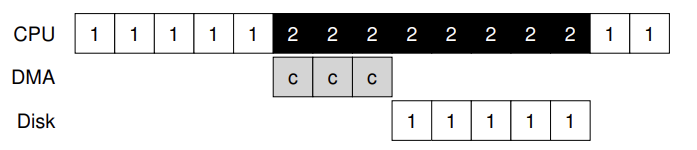
\includegraphics[width=\textwidth]{src/dma.png}
        \caption{Con DMA}
    \end{subfigure}
\end{figure}   

\subsection{Comunicación con dispositivos}

Con el tiempo, se han desarrollado dos métodos principales de comunicación con los dispositivos. El primer método más antiguo es \colorbox{yellow!20}{tener instrucciones de I/O explícitas}. Estas instrucciones especifican una forma para que el SO envíe datos a registros específicos de dispositivos y así, permitir la construcción de los protocolos descritos. Estas instrucciones suelen ser privilegiadas. El SO controla los dispositivos y, por lo tanto, el SO es la única entidad a la que se le permite comunicarse directamente con ellos.

El segundo método para interactuar con los dispositivos se conoce como \colorbox{yellow!20}{I/O mapeado en memoria} (memory mapped I/O). Con este enfoque, el hardware hace que \colorbox{yellow!20}{los registros de dispositivos estén disponibles} como si fueran \colorbox{yellow!20}{ubicaciones de memoria}. Para acceder a un registro en particular, el SO emite una lectura (load) o escritura (store)  en la dirección; el hardware luego enruta la llamada a load/store al dispositivo en lugar de a la memoria principal.

\subsection{El controlador de dispositivo o Device Driver}

En esta parte se plantea una forma de incorporar dispositivos que tienen interfaces muy específicas manteniendo la \colorbox{yellow!20}{generalidad} y mantener \colorbox{yellow!20}{neutral} al SO ante la mayoria de dispositivos. Este problema se resuelve con una \textbf{abstracción}. En el nivel más bajo, una pieza de software en el SO debe conocer en detalle \colorbox{yellow!20}{cómo funciona} un dispositivo. A este software lo llamamos \colorbox{yellow!20}{controlador de dispositivo} (device driver), y cualquier detalle de la interacción del dispositivo está encapsulado dentro.

\begin{floatingfigure}[r]{0.5\textwidth}
    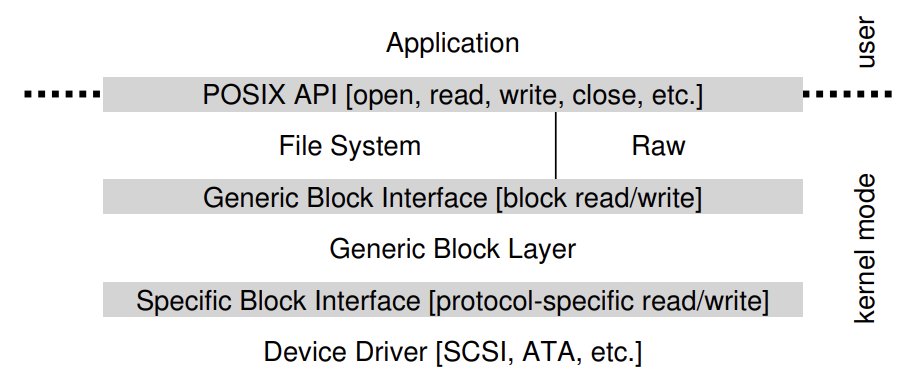
\includegraphics[width=0.5\textwidth]{src/fs.png}
    \caption{Stack del FS en linux}
\end{floatingfigure}

En la figura se puede ver el diagrama simplificado de un sistema de archivos que es completamente ajeno a los detalles de qué clase de disco está usando; simplemente \colorbox{yellow!20}{emite solicitudes} de lectura y escritura de bloques a la capa de bloques genéricos, que las \colorbox{yellow!20}{envía al controlador} de dispositivo apropiado, el cual \colorbox{yellow!20}{maneja los detalles de la emisión} de la solicitud específica.

El diagrama también muestra un interfaz en crudo a los dispositivos, lo que permite aplicaciones especiales para leer y escribir bloques directamente sin utilizar la abstracción de archivos.

\newpage
\subsection{Discos Rotacionales}

El disco consiste en un gran número de \colorbox{yellow!20}{sectores} (bloques de 512-bytes), donde cada uno puede \textit{ser leído} o \textit{escrito}. Están numerados de \colorbox{yellow!20}{0 a N-1}, donde N es el número total de \colorbox{yellow!20}{sectores en el disco}. Se puede asumir que el acceso a dos bloques cercanos dentro del espacio de direcciones del disco será más rápido que el acceso a dos bloques que están más distantes. También se puede asumir que el acceso a bloques en un fragmento contiguo (es decir, una lectura o escritura secuencial) es el modo de acceso más rápido, y generalmente mucho más rápido que cualquier patrón de acceso más aleatorio.

\begin{floatingfigure}[l]{0.3\textwidth}
    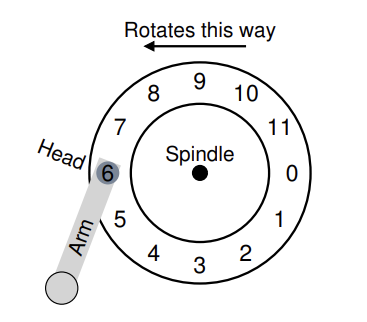
\includegraphics[width=0.3\textwidth]{src/hdd.png}
    \caption{Disco rotacional con una pista}
\end{floatingfigure}

Llamamos \colorbox{yellow!20}{plato} a una superficie circular dura en la que los datos se almacenan de manera persistente mediante la inducción de cambios magnéticos en ella. Un disco puede tener uno o más platos; \colorbox{yellow!20}{cada plato tiene 2 lados}, cada uno de los cuales se llama \colorbox{yellow!20}{superficie}. Los platos están unidos alrededor del eje, que está conectado a un motor que hace girar los platos a una velocidad constante (cuya especificación nos da el \colorbox{yellow!20}{RPM} del disco). 

Los datos se \colorbox{yellow!20}{codifican en cada superficie} en círculos concéntricos de sectores llamados \colorbox{yellow!20}{pistas}. Una sola superficie contiene muchos miles de pistas, estrechamente juntas, con cientos de pistas cabiendo en el ancho de un cabello humano. 

Para \colorbox{yellow!20}{leer y escribir} en la superficie, hay un \colorbox{yellow!20}{cabezal} de disco por cada superficie de la unidad. El cabezal del disco está unido a un solo brazo de disco, que se mueve a través de la superficie para \colorbox{yellow!20}{posicionar el cabezal} sobre la pista deseada.

En la figura, el cabezal del disco, que está unido al extremo del brazo, está posicionado sobre el sector 6, y la superficie está girando en sentido antihorario. Y el funcionamiento es el siguiente: el disco solo debe esperar a que el sector deseado gire y pase debajo del cabezal del disco. Esta espera ocurre con suficiente frecuencia en los discos modernos y es un componente lo suficientemente importante del tiempo de servicio de E/S, que tiene un nombre especial: \colorbox{yellow!20}{retraso rotacional}.

\begin{floatingfigure}[r]{0.6\textwidth}
    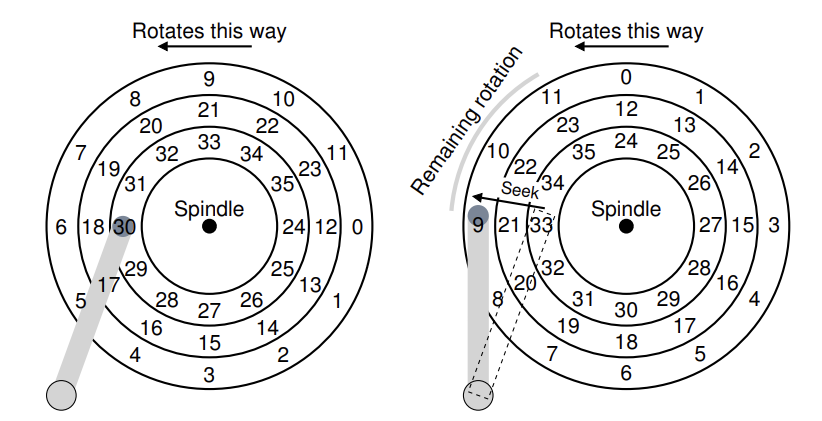
\includegraphics[width=0.6\textwidth]{src/hdd3.png}
    \caption{Disco rotacional con 3 pistas}
\end{floatingfigure}

Los discos modernos tienen millones de pistas, así que sería importante comprender el sistema en un disco multipista. En la figura, el cabezal está actualmente posicionado sobre la pista más interna (que contiene los sectores 24 a 35); la siguiente pista contiene el siguiente conjunto de sectores (12 a 23), y la pista más externa contiene los primeros sectores (0 a 11).

Supongamos que se desea acceder al sector 11: la unidad primero tiene que mover el brazo del disco a la pista correcta (en este caso, la más externa), en un proceso conocido como búsqueda (\colorbox{yellow!20}{seek}). Ahora bien, durante la búsqueda, el brazo se ha movido a la pista deseada, y el plato, por supuesto, ha girado, en este caso aproximadamente 3 sectores. Por lo tanto, el sector 9 está a punto de pasar bajo el cabezal del disco, y solo tenemos que soportar un breve \colorbox{yellow!20}{retraso rotacional} para completar la transferencia. Cuando el sector 11 pase bajo el cabezal del disco, tendrá lugar la fase final de la E/S, conocida como la \colorbox{yellow!20}{transferencia}, \textit{donde los datos se leen desde o se escriben en la superficie}. 

\subsubsection{Consideraciones adicionales}
\begin{itemize}
    \item Muchos discos emplean algún tipo de sesgo de pista para asegurar que las lecturas secuenciales puedan atenderse adecuadamente incluso al cruzar los límites de las pistas. Los sectores a menudo se sesgan de esta manera porque, al cambiar de una pista a otra, el disco necesita tiempo para reposicionar el cabezal (incluso en pistas adyacentes). Sin este sesgo, el cabezal se movería a la siguiente pista, pero el siguiente bloque deseado ya habría girado bajo el cabezal, y así el disco tendría que esperar casi todo el retraso rotacional para acceder al siguiente bloque.
    \item Las pistas externas tienden a tener más sectores que las pistas internas, lo cual es resultado de la geometría; simplemente hay más espacio en las pistas exteriores. Estas pistas se conocen comúnmente como unidades de disco con zonas múltiples, donde el disco se organiza en múltiples zonas y donde una zona es un conjunto consecutivo de pistas en una superficie. Cada zona tiene el mismo número de sectores por pista, y las zonas exteriores tienen más sectores que las zonas interiores.
    \item Una parte importante de cualquier disco moderno es su caché, a veces llamada por razones históricas un búfer de pista. Esta caché es solo una pequeña cantidad de memoria (generalmente alrededor de 8 o 16 MB) que la unidad puede usar para almacenar datos leídos o escritos en el disco. Por ejemplo, al leer un sector del disco, la unidad podría decidir leer todos los sectores de esa pista y almacenarlos en su memoria; al hacerlo, la unidad puede responder rápidamente a cualquier solicitud subsiguiente a la misma pista.
\end{itemize}

\subsubsection{Análisis del tiempo de E/S}
\begin{itemize}
    \item \textbf{Tiempo rotacional:} supongamos que \colorbox{yellow!20}{nos dan las revoluciones por minuto} (RPM) del disco, y queremos calcular el tiempo en ms que toma una rotación. Un mínuto tiene 60 segundos, por lo tanto, sea $x$ el RPM, el tiempo de rotación se puede escribir como:
    \begin{empheq}[box=\fbox]{equation*}
        \frac{60}{x} \cdot 1000 = \_\_\_ ms \text{ por rotación}
    \end{empheq}
    \item \textbf{Tiempo de transferencia:} para esto se tiene una regla de tres simple, si nos dan que la tasa de transferencia es de $y$ MB/s, y queremos calcular el tiempo que toma transferir $z$ MB, se puede escribir como:
    \begin{empheq}[box=\fbox]{equation*}
        \frac{z}{y} \cdot 1000 = \_\_\_ ms
    \end{empheq}
    \item \textbf{Tiempo de lectura/escritura:} Supongamos que se quiere leer los sectores 6,7 y 8, tendriamos 3 etapas para posicionar el cabezar y leer, primero el cabezal comenzó posicionado en el sector 29, para llegar a la pista 6, primero debe \colorbox{yellow!20}{moverse de pista}, luego \colorbox{yellow!20}{esperar} que quede por encima del sector deseado y por último el tiempo en el que se realiza la lectura de los sectores deseados, todo esto va a conformar el \colorbox{yellow!20}{tiempo de E/S}.
    \begin{figure}[h]
        \centering
        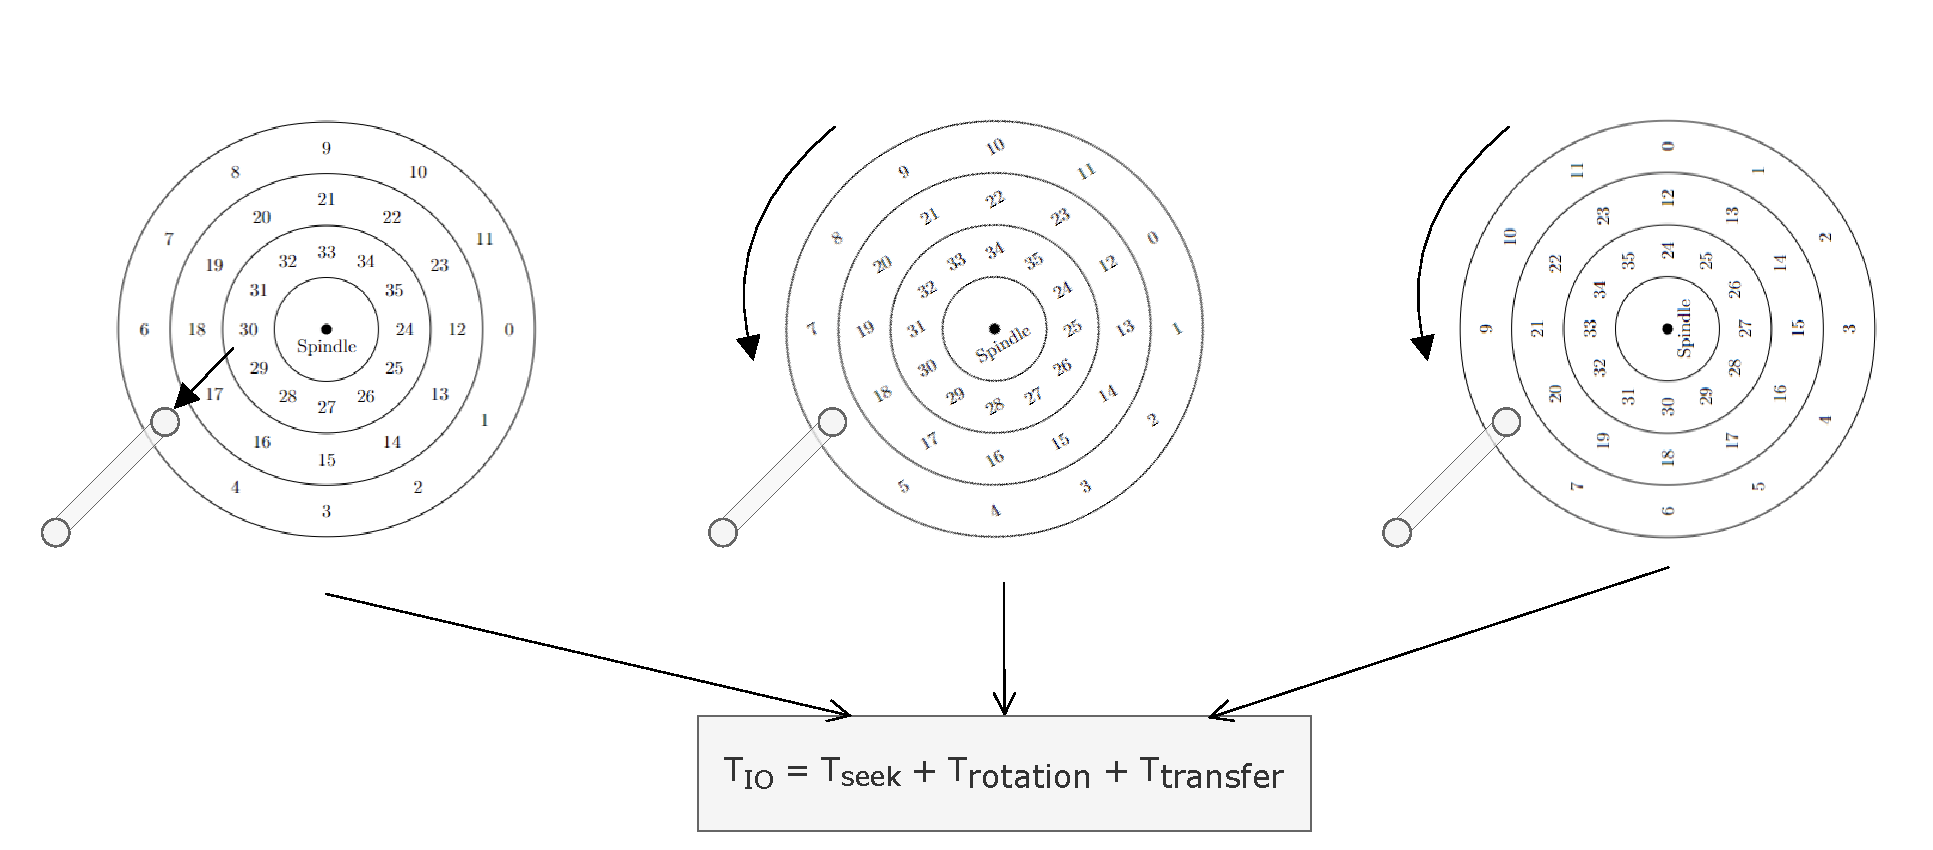
\includegraphics[width=1\textwidth]{src/hdd5.pdf}
    \end{figure}
    \item \textbf{Tasa de transferencia:} la tasa de transferencia para bloques de un determinado tamaño se puede calcular con la siguiente fórmula:
    \begin{empheq}[box=\fbox]{equation*}
        R_{I/O} = \frac{SIZE_{Transfer}}{T_{IO}} 
    \end{empheq}
\end{itemize}

\newpage
\subsection{Planificación del disco}
En la planificación de disco, podemos hacer una buena \colorbox{yellow!20}{estimación del tiempo} que tomará una \colorbox{yellow!20}{tarea}. Estimando el \colorbox{yellow!20}{tiempo de búsqueda} y el posible \colorbox{yellow!20}{retraso rotacional} de una solicitud, el planificador de disco puede saber cuánto tardará cada solicitud y, por lo tanto, escoger la que tomará menos tiempo en atender primero. El planificador de disco intentará seguir el \textbf{principio de SJF} (tarea más corta primero) en su operación.
\subsubsection{SSTF (Shortest Seek Time First)}
Ordena la cola de solicitudes de E/S por pista, \colorbox{yellow!20}{eligiendo primero} las solicitudes en la \colorbox{yellow!20}{pista más cercana}. Por ejemplo, asumiendo que la posición actual del cabezal está sobre la pista interna, y tenemos solicitudes para los sectores 21 (pista media) y 2 (pista externa), entonces emitiríamos la solicitud al sector 21 primero, esperaríamos a que se complete, y luego emitiríamos la solicitud al sector 2. Supongamos que en ejemplo anterior que hubiera un flujo constante de solicitudes a la pista interna, donde el cabezal está actualmente posicionado. Las solicitudes a otras pistas serían \colorbox{yellow!20}{completamente ignoradas} con un enfoque SSTF puro. Este problema es conocido como \colorbox{yellow!20}{starvation}.

\subsubsection{Elevador (SCAN)}
Este algoritmo, se basa en \colorbox{yellow!20}{moverse de un lado a otro} del disco atendiendo solicitudes en orden a lo largo de las pistas. Llamemos a un solo recorrido del disco \colorbox{yellow!20}{un barrido}. Así, si llega una solicitud para un bloque en una pista que ya ha sido atendida en este barrido del disco, no se atiende de inmediato, sino que \textit{se coloca en cola hasta el próximo barrido (en la otra dirección)}. Se dice elevador, ya que se comporta como un elevador que sube o baja y no solo atiende solicitudes de pisos basándose en cuál está más cerca. La desventada de este enfoque, es que \colorbox{yellow!20}{ignora los costos rotacionales del disco}.

\subsubsection{SPTF (Shortest Positioning Time First)}

\begin{floatingfigure}[r]{0.3\textwidth}
    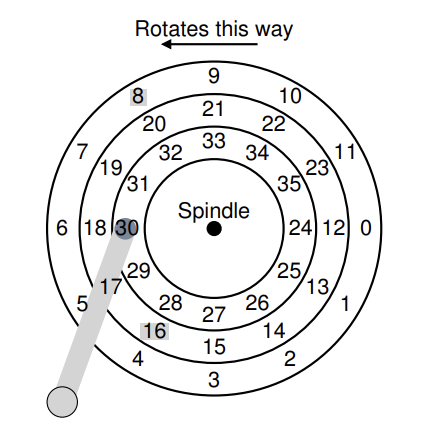
\includegraphics[width=0.3\textwidth]{src/hdd6.png}
    \caption{Ejemplo para planificar}
\end{floatingfigure}

En el ejemplo, el cabezal está sobre el sector 30 en la pista interna. Así que el planificador debe decidir: \textit{¿debe programar el sector 16 o el sector 8 para su próxima solicitud?} En este enfoque, esta decisión depende del \colorbox{yellow!20}{tiempo relativo de búsqueda} en comparación con la rotación. Si, en nuestro ejemplo, el tiempo de búsqueda es mucho mayor que el retraso rotacional, entonces SSTF está bien. Sin embargo, supongamos que la búsqueda es bastante más rápida que la rotación. Entonces, tendría más sentido buscar más lejos para atender la solicitud del sector 8 en la pista externa que realizar una búsqueda más corta a la pista media para atender el sector 16, que tendría que rotar hasta pasar por debajo del cabezal del disco.

\newpage
\section{Archivos y directorios}
La \colorbox{yellow!20}{abstracción de archivo}, consiste en un arreglo lineal de bytes, cada uno de los cuales se puede leer o escribir. Cada archivo tiene algún tipo de nombre de bajo nivel, generalmente un número de algún tipo; a menudo, el usuario no es consciente de este nombre, este nombre es el número del \colorbox{yellow!20}{inodo}. La responsabilidad del sistema de archivos es simplemente \colorbox{yellow!20}{almacenar} dichos datos de forma \colorbox{yellow!20}{persistente} en el disco y asegurarse de que cuando se vuelvan a solicitar los datos, se tenga lo que se puso allí en primer lugar.

\begin{floatingfigure}[r]{0.4\textwidth}
    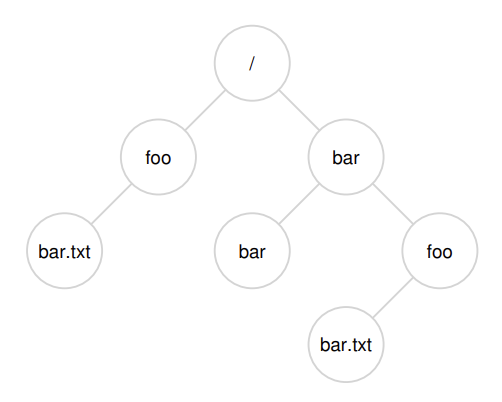
\includegraphics[width=0.4\textwidth]{src/dir.png}
    \caption{Arbol de directorios}
\end{floatingfigure}

La \colorbox{yellow!20}{abstracción de directorio}, al igual que un archivo, también tiene un nombre de bajo nivel (es decir, un número de inodo), pero su contenido es bastante específico: contiene una lista de pares (\colorbox{yellow!20}{nombre legible} por el usuario, \colorbox{yellow!20}{nombre} de \colorbox{yellow!20}{bajo} \colorbox{yellow!20}{nivel}). \textbf{Cada entrada en un directorio se refiere a archivos u otros directorios}. Al colocar directorios dentro de otros directorios, los usuarios pueden construir un \colorbox{yellow!20}{árbol} de directorios arbitrario, bajo el cual se almacenan todos los archivos y directorios. 

La jerarquía de directorios comienza en un directorio raíz (en sistemas basados en UNIX, el directorio raíz se denomina simplemente /) y usa algún tipo de separador para nombrar los subdirectorios posteriores hasta que se nombra el archivo o directorio deseado. El nombre del archivo en este ejemplo a menudo tiene dos partes: bar y txt, separadas por un punto. La primera parte es un nombre arbitrario, mientras que la segunda parte del nombre del archivo generalmente se usa para indicar el tipo de archivo.

\subsection{La interfaz de archivos}

\subsubsection{Crear un archivo}

\begin{enumerate}
    \item Una forma es hacerlo mediante la system call \textbf{open} (pasándole el flag \texttt{O\_CREAT}), que toma un nombre de archivo y devuelve un descriptor de archivo. 
    \begin{tcblisting}{colback=brown!5, colframe=brown!40!black, listing only, listing options={language=C, keywordstyle=\color{blue!35!white}\bfseries}}
    int fd = open("foo", O_CREAT|O_WRONLY|O_TRUNC, S_IRUSR|S_IWUSR);
    \end{tcblisting}
    Los demás flags son para indicar que se desea crear un archivo, escribir en él y truncar el archivo si ya existe. Los flags de permisos indican que el archivo debe ser accesible para lectura y escritura por el usuario que lo creó.
    \item La otra forma de crear un archivo es mediante la system call \textbf{creat}, que es simplemente un envoltorio para open.
    \begin{tcblisting}{colback=brown!5, colframe=brown!40!black, listing only, listing options={language=C, keywordstyle=\color{blue!35!white}\bfseries}}
    int fd = creat("foo", S_IRUSR|S_IWUSR);
    \end{tcblisting}
\end{enumerate}

\subsubsection{Leer y escribir archivos}

\begin{floatingfigure}[r]{0.4\textwidth}
    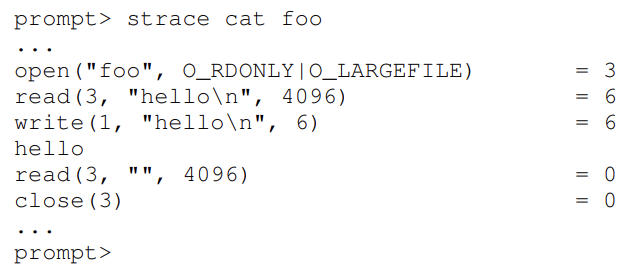
\includegraphics[width=0.4\textwidth]{src/cat.png}
    \caption{Strace de cat}
\end{floatingfigure}

Supongamos que en el archivo foo, esta presente solamente la cadena "hello", luego queremos mostrar por pantalla lo que hay en ese archivo, esto lo hacemos mediante \texttt{cat}.

Lo que hace \texttt{cat} primero es \colorbox{yellow!20}{abrir} el archivo con el flag de \texttt{O\_RDONLY} (solamente lectura), luego esta llamada devuelve el descriptor de archivo $3$ (ya que 0,1,2 son los descriptores de archivo estándar), luego \colorbox{yellow!20}{lee} el archivo con la llamada \texttt{read()}. El primer argumento de read() es el \colorbox{yellow!20}{descriptor} de archivo, lo que indica al sistema de archivos qué archivo debe leerse. El segundo argumento apunta a un \colorbox{yellow!20}{búfer} donde se colocará el resultado de \texttt{read()}. El tercer argumento es el \colorbox{yellow!20}{tamaño del búfer}, que en este caso es de 4 KB. La llamada a read() también retorna exitosamente, aquí devolviendo el número de \colorbox{yellow!20}{bytes leídos}. Por último, escribe en la salida estándar, intenta leer más pero no quedan bytes en el archivo y por último cierra el archivo con \texttt{close()}.

\begin{enumerate}
    \item \textbf{Leer archivos:} para leer un archivo, se usa la system call \textbf{read}, que toma un descriptor de archivo, un búfer y un tamaño de búfer, y devuelve el número de bytes leídos.
    \begin{tcblisting}{colback=brown!5, colframe=brown!40!black, listing only, listing options={language=C, keywordstyle=\color{blue!35!white}\bfseries}}
    char buf[4096];
    int n = read(fd, buf, sizeof(buf));
    \end{tcblisting}
    \item \textbf{Escribir archivos:} para escribir un archivo, se usa la system call \textbf{write}, que toma un descriptor de archivo, un búfer y un tamaño de búfer, y devuelve el número de bytes escritos.
    \begin{tcblisting}{colback=brown!5, colframe=brown!40!black, listing only, listing options={language=C, keywordstyle=\color{blue!35!white}\bfseries}}
    char buf[4096] = "hello";
    int n = write(fd, buf, sizeof(buf));
    \end{tcblisting}
\end{enumerate}

\subsubsection{Leer y escribir archivos con un desplazamiento}
Leer y escribir con un desplazamiento hace referencia a poder manejarlos desde un punto en específico sin tomar desde el \colorbox{yellow!20}{principio hasta el final}. Para hacer esto, se usa la system call \myverb[blue]{lseek}, que toma como primer argumento, un \colorbox{yellow!20}{descriptor de archivo}, como segundo argumento el \colorbox{yellow!20}{desplazamiento} y el tercer argumento, llamado \colorbox{yellow!20}{whence}, determina cómo se realizará la busqueda:
\begin{itemize}
    \item \textbf{SEEK\_SET:} el desplazamiento se establece en el valor de \textit{offset}.
    \item \textbf{SEEK\_CUR:} el desplazamiento se establece en su valor actual más \textit{offset}.
    \item \textbf{SEEK\_END:} el desplazamiento se establece en el tamaño del archivo más \textit{offset}.
\end{itemize}

Entonces hay dos formas de tocar el desplazamiento, la primera es cuando se realiza una lectura o escritura de N bytes, se agrega N al desplazamiento actual; así, cada lectura o escritura actualiza implícitamente el desplazamiento. La segunda es explícitamente con lseek.

En xv6, por ejemplo, la estructura de un archivo es de la siguiente manera:
\begin{tcblisting}{colback=brown!5, colframe=brown!40!black, listing only, listing options={language=C, keywordstyle=\color{blue!35!white}\bfseries}}
struct file {
    int ref;
    char readable;
    char writable;     
    struct inode *ip;  // Inode of file
    uint off;          // Current offset in file
};
\end{tcblisting}    
Y al igual que los procesos, los archivos también se guardan en una tabla de archivos abiertos, que es un arreglo de estructuras de archivos.

\subsection{Entradas compartidas en la tabla de archivos}

Si dos procesos tienen abierto el mismo archivo al mismo tiempo, \colorbox{yellow!20}{cada uno} tendrá su \colorbox{yellow!20}{propia entrada} a la tabla de archivos, de esta manera, cada lectura o escritura lógica de un archivo es independiente y cada proceso \colorbox{yellow!20}{tiene su propio desplazamiento} actual mientras accede al archivo dado. Sin embargo hay casos donde una entrada en la tabla de archivos abiertos es compartida. 
\newpage
\begin{floatingfigure}[r]{0.4\textwidth}
    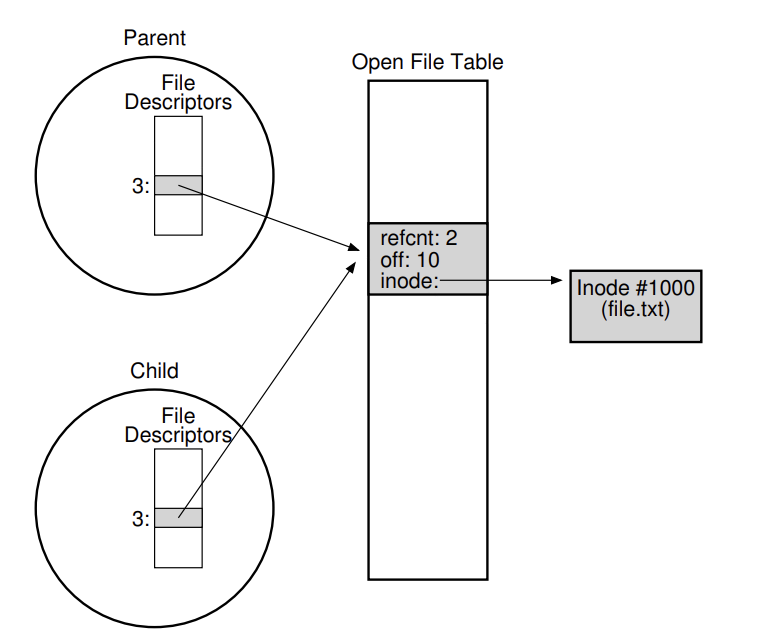
\includegraphics[width=0.4\textwidth]{src/ftc.png}
    \caption{Entradas compartidas}
\end{floatingfigure}

Cuando se crea un proceso hijo con \colorbox{yellow!20}{fork()}, se copia la tabla de archivos abiertos del proceso padre al hijo. Si el hijo y el padre comparten un archivo, entonces \colorbox{yellow!20}{ambos tendrán una entrada} en la tabla de archivos abiertos que apunta al mismo archivo. En este caso, si el padre o el hijo mueven el desplazamiento, el otro proceso verá el cambio, ya que ambos comparten la misma entrada en la tabla de archivos abiertos. Supongamos que el padre crea un proceso hijo, y en ese proceso hijo, se cambia mediante \texttt{lseek()}, el desplazamiento, ese cambio se verá reflejado en el padre también.

Otro caso en el que ocurre esto es con la llamada al sistema \colorbox{yellow!20}{dup()} (y sus variantes dup2() y dup3()). La llamada \texttt{dup()} permite a un proceso crear un nuevo descriptor de archivo que hace referencia al mismo archivo abierto subyacente que un descriptor existente. 

\subsection{Escritura con \texttt{fsync()}}

La mayoría de las veces, cuando un programa llama a \texttt{write()}, simplemente le está diciendo al sistema de archivos que escriba tales datos en el almacenamiento persistente en algún momento en el futuro. Por razones de rendimiento, el sistema de archivos \colorbox{yellow!20}{almacenará temporalmente} estas escrituras en memoria durante un tiempo. 

Algunas aplicaciones requieren una garantía de que los datos se han escrito en el almacenamiento, para esto se llama a \colorbox{yellow!20}{fsync()}. Cuando un proceso llama a fsync() para un descriptor de archivo específico, el sistema de archivos responde forzando todos los datos pendientes (es decir, aún no escritos) al disco para el archivo referido por el descriptor de archivo especificado. La función fsync() \colorbox{yellow!20}{devuelve} una vez que todas estas escrituras \colorbox{yellow!20}{se han completado}.

\subsection{Renombrar y eliminar archivos}

\begin{enumerate}
    \item \textbf{Renombrar archivos:} para renombrar un archivo, se usa la system call \myverb[blue]{rename}, que toma dos nombres de archivo y cambia el nombre del primer archivo al segundo.
    \begin{tcblisting}{colback=brown!5, colframe=brown!40!black, listing only, listing options={language=C, keywordstyle=\color{blue!35!white}\bfseries}}
    rename("foo", "bar");
    \end{tcblisting}
    \item \textbf{Eliminar archivos:} para eliminar un archivo, se usa la system call \myverb[blue]{unlink}, que toma un nombre de archivo y lo elimina del sistema de archivos.
    \begin{tcblisting}{colback=brown!5, colframe=brown!40!black, listing only, listing options={language=C, keywordstyle=\color{blue!35!white}\bfseries}}
    unlink("foo");
    \end{tcblisting}
\end{enumerate}

\subsection{Obtener información sobre archivos}

Para ver los metadatos de un archivo, se usa la system call \myverb[blue]{stat()} o \myverb[blue]{fstat()}, estas llamadas toman como parámetro un nombre de archivo o un descriptor de archivo y llena una estructura con información sobre el archivo: 
\begin{tcblisting}{colback=brown!5, colframe=brown!40!black, listing only, listing options={language=C, keywordstyle=\color{blue!35!white}\bfseries}}
struct stat {
    dev_t st_dev;         // ID of device containing file
    ino_t st_ino;         // inode number
    mode_t st_mode;       // protection
    nlink_t st_nlink;     // number of hard links
    uid_t st_uid;         // user ID of owner
    gid_t st_gid;         // group ID of owner
    dev_t st_rdev;        // device ID (if special file)
    off_t st_size;        // total size, in bytes
    blksize_t st_blksize; // blocksize for filesystem I/O
    blkcnt_t st_blocks;   // number of blocks allocated
    time_t st_atime;      // time of last access
    time_t st_mtime;      // time of last modification
    time_t st_ctime;      // time of last status change
};
\end{tcblisting}        

\subsection{Crear, leer y eliminar directorios}

\begin{enumerate}
    \item \textbf{Crear directorios:} para crear un directorio, se usa la system call \myverb[blue]{mkdir}, que toma un nombre de directorio y crea un directorio con ese nombre.
    \begin{tcblisting}{colback=brown!5, colframe=brown!40!black, listing only, listing options={language=C, keywordstyle=\color{blue!35!white}\bfseries}}
    mkdir("foo", 0755);
    \end{tcblisting}
    El segundo argumento es un número octal que indica los permisos del directorio.
    \item \textbf{Leer directorios:} para leer un directorio, se usa la system call \myverb[blue]{opendir}, que toma un nombre de directorio y devuelve un puntero a una estructura de directorio.
    \begin{tcblisting}{colback=brown!5, colframe=brown!40!black, listing only, listing options={language=C, keywordstyle=\color{blue!35!white}\bfseries}}
    DIR *d = opendir("foo");
    \end{tcblisting}
    Podemos también leer el contenido del directorio con \myverb[blue]{readdir()}, nos devuelve un puntero a una estructura de directorio.
    \begin{tcblisting}{colback=brown!5, colframe=brown!40!black, listing only, listing options={language=C, keywordstyle=\color{blue!35!white}\bfseries}}
    struct dirent {
        char d_name[256]; // filename
        ino_t d_ino; // inode number
        off_t d_off; // offset to the next dirent
        unsigned short d_reclen; // length of this record
        unsigned char d_type; // type of file
    };
    \end{tcblisting}
    \item \textbf{Eliminar directorios:} para eliminar un directorio, se usa la system call \myverb[blue]{rmdir}, que toma un nombre de directorio y lo elimina del sistema de archivos.
    \begin{tcblisting}{colback=brown!5, colframe=brown!40!black, listing only, listing options={language=C, keywordstyle=\color{blue!35!white}\bfseries}}
    rmdir("foo");
    \end{tcblisting}
    Si se intenta eliminar un directorio que no está vacío, la llamada a rmdir() fallará.
\end{enumerate}

\subsection{Hard links y Symbolic links}

\begin{enumerate}
    \item Un enlace duro (\colorbox{yellow!20}{hard link}) es una referencia directa a un archivo a través de su inodo. Al utilizar un enlace duro, se puede cambiar el contenido o la ubicación del archivo referenciado ya que su inodo sigue apuntando al mismo archivo.
    \item Los enlaces simbólicos (\colorbox{yellow!20}{soft links}) son simplemente archivos que contienen un nombre de archivo. Cuando se accede a un symbolic link, el sistema de archivos lo sigue y accede al archivo al que apunta. Los symbolic links son útiles para crear atajos a archivos o directorios, o para crear enlaces a archivos en otros sistemas de archivos. 
\end{enumerate}

Cuando se crea un archivo, primero, se está creando una estructura (el inodo) que rastreará casi toda la información relevante sobre el archivo, y segundo, se está enlazando un nombre legible por humanos a ese archivo y poniendo ese enlace en un directorio. Este enlace entre un nombre y un inodo es un enlace duro. 

\begin{enumerate}
    \item Para crear un enlace duro, se usa la system call \myverb[blue]{link}, que toma dos nombres de archivo y crea un nuevo enlace al archivo referido por el primer nombre.
    \item Para crear un enlace simbólico, se usa la system call \myverb[blue]{symlink}, que toma dos nombres de archivo y crea un nuevo enlace simbólico al archivo referido por el primer nombre.
\end{enumerate}

\subsection{Permisos y control de acceso a archivos}
En la consola, para ver los permisos de un archivo, se usa el comando \texttt{ls -l}, que muestra los permisos de los archivos en el directorio actual. Los permisos de un archivo se dividen en tres gru   pos: \colorbox{yellow!20}{propietario}, \colorbox{yellow!20}{grupo} y \colorbox{yellow!20}{otros}. Cada grupo tiene tres permisos: \colorbox{yellow!20}{lectura}, \colorbox{yellow!20}{escritura} y \colorbox{yellow!20}{ejecución}.

\begin{figure}[h]
    \centering
    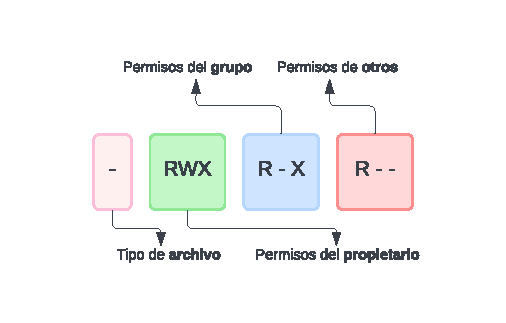
\includegraphics[width=0.7\textwidth]{src/perms.pdf}
    \caption{Permisos de archivos}
\end{figure}

\subsection{Operaciones de inodos}

\begin{itemize}
    \item \myverb[blue]{stat()} y \myverb[blue]{fstat()}: obtienen información sobre un archivo.
    \item \myverb[blue]{link()}: crea un enlace duro a un archivo.
    \item \myverb[blue]{unlink()}: elimina un enlace duro a un archivo.
    \item \myverb[blue]{symlink()}: crea un enlace simbólico a un archivo.
    \item \myverb[red]{mkdir()}: crea un directorio.
    \item \myverb[red]{mknod()}: crea un archivo especial.
    \item \myverb[green]{rename()}: renombra un archivo.
    \item \myverb[green]{truncate()}: cambia el tamaño de un archivo. Aumenta, disminuye o mantiene el tamaño del archivo.  
\end{itemize}

\newpage

\section{Implementación de un sistema de archivos}

Hay dos aspectos clave que hay que comprender de un sistema de archivos (FS \textit{filesystem}):

\begin{enumerate}
    \item \textbf{Estructuras de datos}: Los primeros sistemas de archivos emplean estructuras simples, como \colorbox{green!20}{arreglos} de bloques u otros objetos, mientras que sistemas de archivos más sofisticados, como el \textit{XFS} de \textit{SGI}, usan estructuras más complejas basadas en \colorbox{green!20}{árboles}.
    \item \textbf{Métodos de acceso}: En este punto se debe evaluar como una función de sistema de archivos, como \texttt{read()} o \texttt{write()}, se \colorbox{green!20}{mapea} a las estructuras de datos subyacentes, al igual de que estructura de datos se leen y escriben durante la ejecución de una llamada al sistema. Y por último la \colorbox{green!20}{eficiencia} de estos pasos.
\end{enumerate}

\subsection{Estructuras de datos}

\begin{floatingfigure}[r]{0.5\textwidth}
    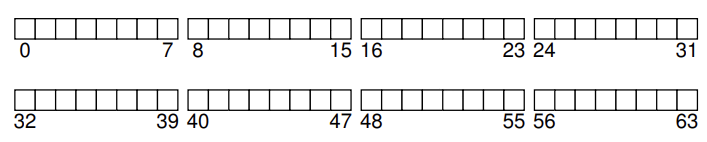
\includegraphics[width=0.5\textwidth]{src/fs1.png}
    \caption{Disco con bloques}
\end{floatingfigure}

Los sistemas de archivo simples, usan \colorbox{green!20}{tamaño} de bloque \colorbox{green!20}{fijo}, tomemos por ejemplo un tamaño de 4kb. En este caso vamos a tener 64 bloques. Ahora hay que analizar el \colorbox{green!20}{qué} poner dentro de dichos bloques. Primeramente vamos a tener la mayor parte del disco con \colorbox{green!20}{datos del usuario}. Para simplificar, digamos que \textbf{56 de los 64 bloques} se van a dedicar a esto. 

Algo que también se debe tener en cuenta es la \colorbox{green!20}{información} sobre cada archivo, pieza clave de los \colorbox{green!20}{metadatos} e información sobre \colorbox{green!20}{qué bloques} de datos conforman un archivo, el \colorbox{green!20}{tamaño}, su \colorbox{green!20}{propietario} y \colorbox{green!20}{derechos} de acceso, los \colorbox{green!20}{tiempos de modificación}, y mas información. Para todo esto, se tiene una estructura llamada \myverb[green]{inode}. El tamaño de los inodes no suele ser muy significativo, suponiendo que tienen un tamaño de 256 bytes, podriamos tener \colorbox{green!20}{16 inodes por bloque}.

Ahora nos faltan las \textbf{estructuras de datos} para rastrear si los inodes o bloques de datos están \colorbox{green!20}{libres} o \colorbox{green!20}{asignados}.

\begin{floatingfigure}[l]{0.5\textwidth}
    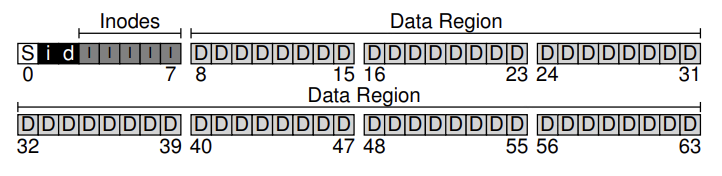
\includegraphics[width=0.5\textwidth]{src/fs2.png}
\end{floatingfigure}

Se va a usar la estructura de \colorbox{green!20}{bitmap}, que es un arreglo de bits, donde cada bit se utiliza para indicar si el bloque u objeto correspondiente está \colorbox{green!20}{libre (0)} o \colorbox{green!20}{en uso (1)}. Por último de alguna forma hay que guardar la cantidad de inodos y bloques de datos que hay en el sistema de archivos, así como donde comienza cada estructura. Para esto se usa un \colorbox{green!20}{superbloque}, que es una estructura que contiene toda esta información. Así el sistema operativo leerá primero el superbloque para inicializar varios parámetros y luego adjuntar el volumen al árbol del sistema de archivos. Cuando se acceden a archivos dentro del volumen, el sistema sabrá exactamente dónde buscar las estructuras necesarias en el disco. Esta estructura se ve en el diagrama \textbf{denotado con una S}.

\subsubsection{Inodos}

Se llama inodo a un \colorbox{green!20}{nodo de índice}, donde cada uno es referido de forma implícita mediante un número. En los sistemas de archivos simples como \textbf{vsfs}, dado un número de inodo, se puede calcular directamente en qué parte del disco se encuentra el inodo correspondiente.

\begin{floatingfigure}[r]{0.6\textwidth}
    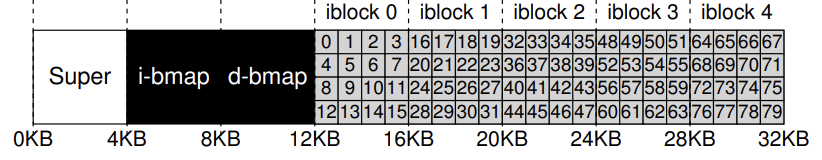
\includegraphics[width=0.6\textwidth]{src/inode.png}
    \caption{Tabla de inodos}
\end{floatingfigure}

Supongamos que se tiene la siguiente estructura donde se puede observar tanto el superbloque como los bitmaps, seguido de los inodos (80 inodos de 256 bytes). 

\textbf{Se busca leer el inodo 32}, lo primero que haria el sistema operativo es calcular el \colorbox{green!20}{offset} en la región de inodos, es decir va a hacer $32 \times \text{sizeof(i-node)}$ en este caso $8192$, luego sumaría esto a la \colorbox{green!20}{dirección de inicio} de la tabla de inodos en el disco. Como los discos trabajan por \textbf{sectores} de 512 bytes, vamos a tener que aplicar una transformación teniendo en cuenta el tamaño de los espacios en memoria.

\begin{align*}
    \text{block} &= (\text{i-number} * \text{sizeof(inode\_t)}) / \text{blockSize}; \\
    \text{sector} &=  ((\text{block} * \text{blockSize}) + \text{inodeStartAddr}) / \text{sectorSize};
\end{align*}

\newpage
Dentro de cada inodo está prácticamente toda la información sobre un archivo: su \colorbox{green!20}{tipo}, su \colorbox{green!20}{tamaño}, el \colorbox{green!20}{número} de bloques asignados, información de \colorbox{green!20}{protección},  información de \colorbox{green!20}{tiempos},  y también información sobre dónde residen sus \colorbox{green!20}{bloques de datos} en el disco. Toda esta información sobre un archivo se llama \textbf{metadatos}.

\begin{figure}[h]
    \centering
    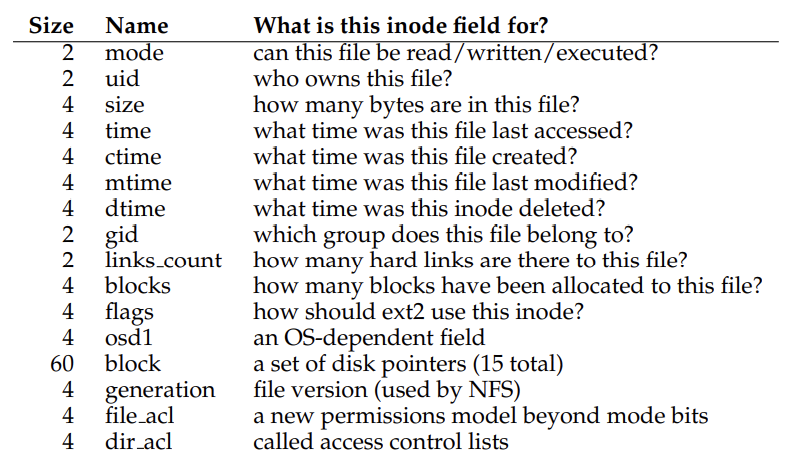
\includegraphics[width=0.7\textwidth]{src/inode1.png}
    \caption{Ext2 inode}
\end{figure}

Una forma de soportar archivos mas grandes, se creó algo llamado \colorbox{green!20}{puntero indirecto}. Entonces se agrega este puntero al inodo, de manera que este puntero se refiere a un bloque que contiene punteros a bloques indirectos, cada uno de los cuales \colorbox{green!20}{contiene punteros} a bloques de datos. Un bloque doble indirecto añade así la posibilidad de \colorbox{green!20}{expandir archivos} con 1024 · 1024 o 1 millón de bloques de 4 KB adicionales, es decir, soportando archivos de más de 4 GB de tamaño. Y cuanto mas tamaño se desee soportar, se agrega por ejemplo un puntero triple indirecto y asi sucesivamente.

De esta forma surge el concepto de \colorbox{green!20}{índice de múltiples niveles} para apuntar a bloques de archivo.

\subsection{Organización de directorios}

Los directorios tienen una organización simple; un directorio contiene una lista de pares \colorbox{green!20}{nombre de entrada}, \colorbox{green!20}{número de inodo}. Para cada archivo o directorio en un directorio dado, hay una cadena y un número en el bloque de datos del directorio. 

\begin{floatingfigure}[r]{0.6\textwidth}
    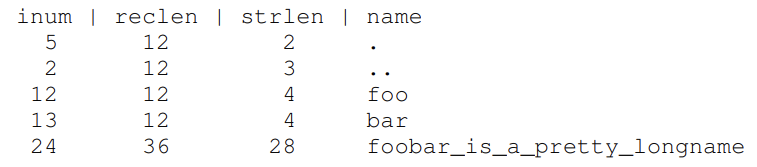
\includegraphics[width=0.6\textwidth]{src/dir1.png}
    \caption{Ejemplo de directorio}
\end{floatingfigure}

En este ejemplo, cada entrada tiene un número de inodo, longitud de registro (el total de bytes para el nombre más cualquier espacio sobrante), longitud de cadena (la longitud real del nombre) y finalmente el nombre de la entrada. Eliminar un archivo (por ejemplo, llamando a unlink()) puede dejar un espacio vacío en medio del directorio, y por lo tanto debería haber alguna manera de marcarlo.

Los sistemas de archivos suelen tratar los directorios como un tipo especial de archivo. Así, un directorio tiene un inodo, en algún lugar de la tabla de inodos (con el campo de tipo del inodo marcado como “directorio” en lugar de “archivo regular”). El directorio tiene bloques de datos a los que apunta el inodo (y quizás, bloques indirectos); estos bloques de datos están en la región de bloques de datos de nuestro sistema de archivos simple. Nuestra estructura en disco permanece sin cambios.

\subsubsection{Métodos de acceso}

Acá nos planteamos la pregunta, que sucede cuando se hace el requerimiento de leer un archivo, por ejemplo supongamos que se hace la llamada \myverb[blue]{open("/foo/bar", O\_REONLY)}, pasaría lo siguiente:

\begin{enumerate}
    \item Buscar el inodo del archivo \texttt{bar} en el directorio \texttt{foo}:
    \begin{enumerate}
        \item Inicia el recorrido en el directorio raíz \colorbox{green!20}{root} del FS (/).
        \item El FS lee el bloque que contiene el inodo del directorio raíz (generalmente el 2).
        \item Se busca en el inodo de la carpeta foo, y se lee el bloque de datos que contiene las entradas de directorio.
        \item Verifica el contenido del inodo foo, buscando la entrada de bar.
    \end{enumerate}
    \item Se verifican los permisos, se asigna un descriptor para el proceso y retorna ese descriptor al usuario.
\end{enumerate}

\subsubsection{Lectura}

Ahora bien, que sucederia si se hace la llamada \myverb[blue]{read(fd, buf, 4096)}: 

\begin{enumerate}
    \item Lectura del primer bloque del archivo, consulta al inodo del archivo bar, buscando la ubicación de dicho bloque.
    \begin{itemize}
        \item Se actualiza la fecha de último acceso del inodo.
        \item Se actualiza el offset en la tabla de archivos abiertos.
    \end{itemize}
\end{enumerate}

Gráficamente el proceso de lectura es el siguiente:

\begin{figure}[h]
    \centering
    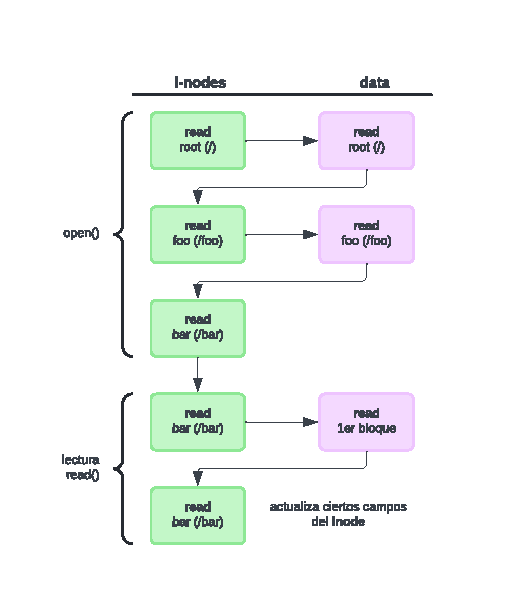
\includegraphics[width=0.7\textwidth]{src/read.pdf}
    \caption{Lectura de un archivo}
\end{figure}

\subsubsection{Escritura}

Al hablar de escritura cambia el enfoque, hay que pensar en que pasa si no está presente el archivo, supongamos que tenemos que hacer la llamada \myverb[blue]{creat("/foo/bar", 0755)}, y luego \myverb[blue]{write(fd)}: 

\begin{enumerate}
    \item Creación del archivo bar en el directorio foo:
    \begin{enumerate}
        \item Leemos el inodo del directorio raíz.
        \item Leemos el bloque de datos para buscar la entrada de directorio foo.
        \item Leemos el inodo de foo.
        \item Leemos el bloque de datos de foo para buscar la entrada de bar.
        \item Como el \textbf{archivo no existe}, se lee y escribe en el bitmap de bloques de datos.
        \item Actualizo el bloque de datos de foo con la nueva entrada de bar.
        \item Leo el inodo de bar y actualizo los metadatos.
        \item Actualizo los metadatos del inodo de foo.
    \end{enumerate}
    \item Actualizar el contenido del archivo:
    \begin{enumerate}
        \item Se puede llegar a requerir la asignación de bloques de datos.
        \item Se generan 5 requerimientos de E/S:
        \begin{itemize}
            \item Lectura del \colorbox{green!20}{data bitmap}.
            \item Escritura del \colorbox{green!20}{data bitmap}.
            \item Lectura y escritura del inodo.
        \end{itemize}
        \item Escritura de los datos en el bloque de datos.
    \end{enumerate}
\end{enumerate}

\begin{figure}[h]
    \centering
    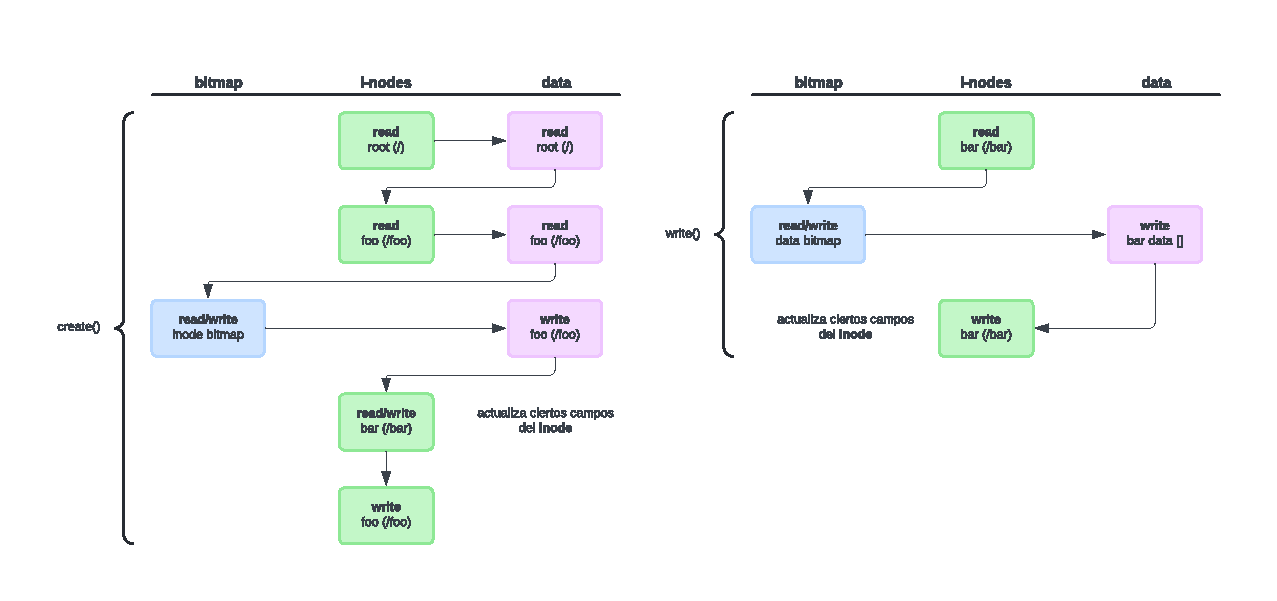
\includegraphics[width=1\textwidth]{src/write.pdf}
    \caption{Escritura de un archivo}
\end{figure}

\subsection{Desempeño de un sistema de archivos}

Como muestran los ejemplos anteriores, leer y escribir archivos puede ser \colorbox{green!20}{costoso}, ya que involucra \colorbox{green!20}{múltiples} \colorbox{green!20}{operaciones} de entrada/salida (I/O) en el disco. Para solucionar lo que claramente sería un problema de rendimiento, la mayoría de los sistemas de archivos \textit{utilizan de forma intensiva la memoria del sistema (DRAM) para almacenar en caché bloques importantes}. 

Esto se basa practicamente en el siguiente concepto, supongamos que estamos constantemente escribiendo y leyendo un inodo, entonces el sistema operativo va a mantener en memoria ese inodo, para evitar tener que ir a buscarlo al disco cada vez que se necesite.

Podemos hacer una distinción entre dos tipos de sistema adoptados por los sistemas de archivos:
\begin{itemize}
    \item Primeros sistemas: \textbf{cache de tamaño fijo}, una porción fija de la memoria se asigna específicamente para la caché del sistema de archivos al arrancar el sistema. La desventaja es que cuando el sistema de archivos no necesita la totalidad de este 10\% de memoria asignada, la memoria permanece sin uso y no puede ser redistribuida a otras aplicaciones o partes del sistema, lo que genera ineficiencia.
    \item Sistemas mas modernos: \textbf{Caché de Páginas Unificada con Partición Dinámica}, la memoria no está particionada estáticamente. En su lugar, se utiliza una partición dinámica que permite que la misma memoria sea compartida entre la caché del sistema de archivos y la memoria virtual (páginas de memoria que las aplicaciones usan para sus datos). Esto permite que el sistema administre la memoria de manera flexible según las necesidades en tiempo real. La misma memoria puede ser utilizada ya sea como caché de archivos o como memoria virtual para aplicaciones. Así, cuando una aplicación requiere más memoria virtual, el sistema puede reducir la caché de archivos y viceversa.
    
    La principal ventaja de este enfoque es la optimización del uso de la memoria total del sistema. Si el sistema de archivos requiere menos memoria en un momento dado, esa memoria se reutiliza para las aplicaciones, evitando desperdicios. De igual forma, si el sistema de archivos requiere más caché (por ejemplo, debido a accesos frecuentes a ciertos archivos), puede obtenerla sin que el rendimiento general del sistema se vea afectado.
\end{itemize}

\begin{table}[htb]
    \refstepcounter{table}\label{tab:mytab}
    \begin{tcolorbox}[tab2,tabularx*={\renewcommand{\arraystretch}{1.5}}{
        >{\centering\arraybackslash}Y|>{\centering\arraybackslash}Y|>{\centering\arraybackslash}Y},title={Tabla \thetable. Tipos de sistemas de archivos},boxrule=0.8pt]
    \textbf{Característica} & \textbf{Caché de Tamaño Fijo} & \textbf{Caché Unificada (Partición Dinámica)} \\\hline\hline
    \textbf{Asignación de Memoria} & Estática al inicio del sistema & Dinámica según demanda \\\hline
    \textbf{Flexibilidad de Uso} & Solo para I/O de sistema de archivos & Uso compartido entre sistema de archivos y memoria virtual \\\hline
    \textbf{Eficiencia} & Memoria no usada por I/O se desperdicia & Maximiza el uso de memoria disponible \\\hline
    \textbf{Impacto en Rendimiento} & Limitada si el sistema de archivos necesita más memoria & Optimizada para adaptarse a necesidades cambiantes \\\hline
    \end{tcolorbox}
\end{table}

\section{Fast File System (FFS)}

El sistema de archivos UNIX original tenía problemas de rendimiento debido a la dispersión de datos en el disco, lo que generaba un alto costo de \colorbox{blue!20}{posicionamiento} y \colorbox{blue!20}{fragmentación}. Los archivos y sus metadatos no estaban organizados para minimizar estos costos, lo que resultaba en una velocidad de acceso significativamente reducida.

Para mejorar el rendimiento, el Fast File System (FFS) fue diseñado considerando la \colorbox{blue!20}{disposición física} del disco. Manteniendo la interfaz de programación original pero optimizando la \colorbox{blue!20}{implementación interna}, FFS abrió paso a sistemas de archivos que adaptan su funcionamiento interno para mejorar la velocidad, confiabilidad y otros factores sin afectar la compatibilidad con aplicaciones. En resumen, se creó un nuevo sistema que manteniendo la interfaz de E/S, modifique las estructuras de datos y las políticas de asignación teniendo en cuenta cómo se almacenan los datos en el disco, mejorando así notablemente el desempeño.

\subsection{Nuevas estructuras de datos}

\begin{floatingfigure}[r]{0.4\textwidth}
    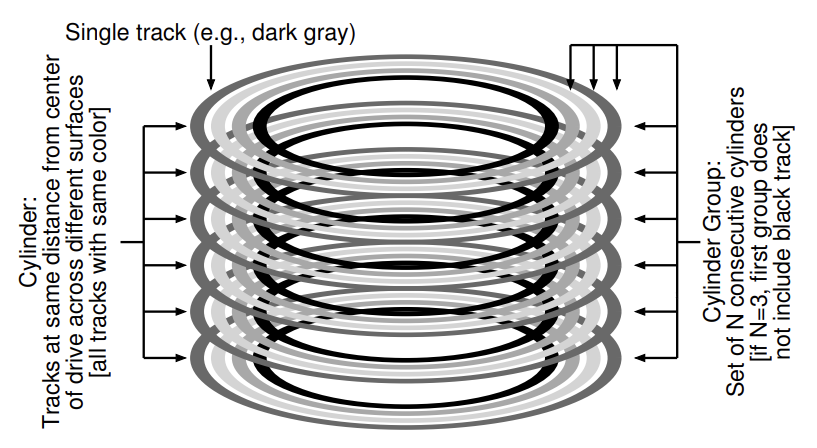
\includegraphics[width=0.4\textwidth]{src/ffs.png}
    \caption{Organización de FFS}
\end{floatingfigure}

FFS organiza el disco en grupos de cilindros, segmentos que agrupan pistas en distintas superficies a la misma distancia del centro del disco. Esta agrupación permite que archivos y directorios relacionados se almacenen cerca unos de otros, reduciendo las búsquedas en el disco y mejorando el rendimiento. Cada grupo contiene inodos, bloques de datos y estructuras para rastrear qué elementos están libres o en uso.

La idea es que, por ejemplo todos los tracks negros que se ven en la figura, puedan ser accedidos en el mismo movimiento, en este caso el tiempo que me demoro en acceder a los datos va a ser el mismo, ya que tomamos en cuenta la tecnología de construcción de los discos duros magnéticos.  Es decir ahora no vamos a ver mas el disco como una estructura lineal desde el bloque 0 hasta el N, sino que vamos a ver el disco como una estructura que va a tener \colorbox{blue!20}{varios grupos} (uno por cilindro). Con esto, el principio de \colorbox{blue!20}{localidad} mejora el desempeño \colorbox{blue!20}{evitando los tiempos de busqueda}.

\newpage

\begin{figure}[h]
    \centering
    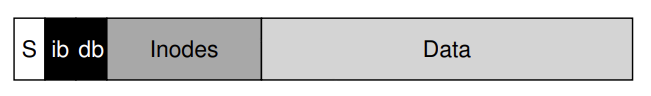
\includegraphics[width=0.8\textwidth]{src/ffs1.png}
    \caption{Estructura de un cilindro}
\end{figure}

Ahora similar a como teniamos antes, vamos a tener esta estructura de datos \colorbox{blue!20}{por cada grupo}. Es decir ahora nuestros \colorbox{blue!20}{inodes} no van a estar mas unificados en una parte del disco sino que estan \colorbox{blue!20}{distribuidos} en todos los cilindros, al igual que los \colorbox{blue!20}{bitmaps}. Y vamos a tener una \colorbox{blue!20}{copia del superbloque} por cada cilindro.

\subsection{Políticas de asignación}

FFS asigna archivos y directorios siguiendo la regla de proximidad. Intenta colocar directorios con \colorbox{blue!20}{pocos} \colorbox{blue!20}{elementos} asignados en grupos con muchos \colorbox{blue!20}{inodos libres}, y asigna los bloques de datos de un archivo en el \colorbox{blue!20}{mismo grupo} que su \colorbox{blue!20}{inodo} para reducir los tiempos de búsqueda. Los archivos dentro de un \colorbox{blue!20}{mismo directorio} se colocan en el \colorbox{blue!20}{mismo grupo}, siempre que sea posible.

\subsubsection{Asignación de archivos muy grandes}

Para evitar que archivos grandes llenen completamente un grupo, FFS divide el archivo en bloques y \colorbox{blue!20}{distribuye} cada "chunk" en diferentes grupos. Aunque esto \colorbox{blue!20}{afecta el rendimiento} en accesos secuenciales, la técnica de \colorbox{blue!20}{amortización} reduce el impacto dividiendo los archivos en bloques lo suficientemente grandes para minimizar las búsquedas entre cada parte.

Además de la organización de datos, FFS introdujo innovaciones de usabilidad como nombres de archivo largos, enlaces simbólicos y la operación atómica rename(). También emplea sub-bloques de 512 bytes para minimizar el desperdicio de espacio en archivos pequeños, aunque evitando costos de reubicación al usar un buffer que permite escribir en bloques de 4 KB en la mayoría de los casos.

\subsubsection{Cálculo del chunksize}
\begin{itemize}
    \item Se busca un ancho de banda pico del 50\%.
    \begin{itemize}
        \item Mitad del tiempo de búsqueda.
        \item Mitad del tiempo de transferencia.
    \end{itemize}
    \item Se tiene un ancho de banda de $xMb/s$ y un tiempo de posicionamiento de $yms$.
    \begin{equation*}
        \frac{x Mb}{sec} \cdot \frac{1024 Kb}{1Mb} \cdot \frac{1 sec}{1000 ms} \cdot y ms = z Kb
    \end{equation*}
    es decir la formula simplemente es $x \cdot 1024 \cdot y / 1000$.
\end{itemize}

\section{Consistencia ante fallos}

El sistema de archivos maneja un conjunto de estructuras de datos para implementar las abstracciones esperadas: archivos, directorios y toda la metadata necesaria para soportar la abstracción básica que esperamos de un sistema de archivos. A diferencia de la mayoría de las estructuras de datos (por ejemplo, las que se encuentran en la memoria de un programa en ejecución), las estructuras de datos de un sistema de archivos deben persistir, es decir, deben mantenerse a largo plazo, almacenadas en dispositivos que retienen datos a pesar de la pérdida de energía (como discos duros o SSDs basados en memoria flash).

Uno de los principales desafíos que enfrenta un sistema de archivos es cómo \colorbox{blue!20}{actualizar estructuras de datos}  \colorbox{blue!20}{persistentes} a pesar de la posible pérdida de energía o de un fallo del sistema.

\subsection{Ejemplo de inconsistencia}

Supongamos que la carga de trabajo es sencilla: la adición de un único bloque de datos a un archivo existente. Esta adición se realiza \colorbox{blue!20}{abriendo} el archivo, llamando a \colorbox{blue!20}{lseek()} para mover el offset del archivo al final del mismo y luego emitiendo una sola escritura de 4KB al archivo antes de cerrarlo. Supongamos también que estamos usando estructuras de sistema de archivos simples en el disco, incluye un bitmap de inodos (con solo 8 bits, uno por inodo), un bitmap de datos (también 8 bits, uno por bloque de datos), inodos (8 en total, numerados del 0 al 7, y distribuidos en cuatro bloques), y bloques de datos (8 en total, numerados del 0 al 7).

\begin{floatingfigure}[r]{0.6\textwidth}
    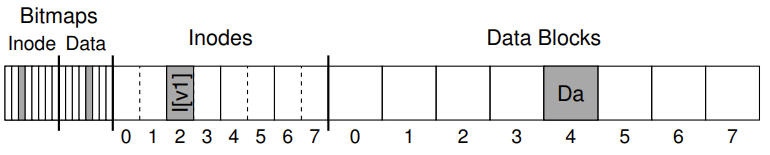
\includegraphics[width=0.6\textwidth]{src/per.png}
    \caption{Ejemplo de inconsistencia}
\end{floatingfigure}

Se puede ver en la figura que que un solo inodo está asignado (el inodo número 2), que está marcado en el bitmap de inodos, y un único bloque de datos asignado (bloque de datos 4), también marcado en el bitmap de datos. El inodo se denota como I[v1], ya que es la primera versión de este inodo; pronto será actualizado. Dentro del inodo se encuentra la siguiente información: el tamaño del archivo (4096 bytes), un puntero directo al bloque de datos 4, y un puntero indirecto que no se utiliza en este ejemplo.
\begin{tcblisting}{colback=brown!5, colframe=brown!40!black, listing only, listing options={language=C, keywordstyle=\color{blue!35!white}\bfseries}}
owner : remzi
permissions : read-write
size : 1
pointer : 4
pointer : null
pointer : null
pointer : null
\end{tcblisting}

El tamaño del archivo es 1 (\colorbox{blue!20}{tiene un bloque asignado}), el primer puntero directo apunta al \colorbox{blue!20}{bloque 4} (el \colorbox{blue!20}{primer bloque} de datos del archivo), y los \colorbox{blue!20}{otros tres} punteros directos están en null (indicando que \colorbox{blue!20}{no están en uso}). 

\begin{floatingfigure}[r]{0.6\textwidth}
    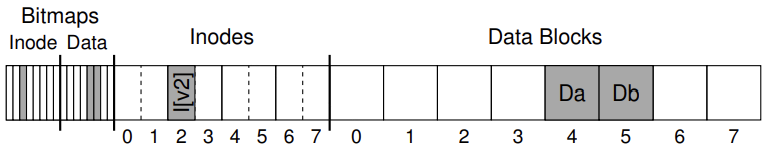
\includegraphics[width=0.6\textwidth]{src/per2.png}
    \caption{Ejemplo de inconsistencia}
\end{floatingfigure}

Cuando añadimos un nuevo bloque de datos al archivo, debemos actualizar tres estructuras en el disco: \colorbox{blue!20}{el inodo} (que debe apuntar al nuevo bloque y registrar el nuevo tamaño aumentado), el \colorbox{blue!20}{nuevo bloque} de datos Db y una nueva versión del \colorbox{blue!20}{bitmap} de datos (llamado B[v2]) para indicar que se ha asignado el nuevo bloque de datos.

\textbf{Para lograr esta transición, el sistema de archivos debe realizar tres escrituras separadas en el disco, una para el inodo (I[v2]), otra para el bitmap (B[v2]) y otra para el bloque de datos (Db). }

Los posibles escenarios de fallo son los siguientes:

\begin{itemize}
    \item \colorbox{blue!20}{Solo el bloque de datos (Db) se escribe en el disco}. En este caso, los datos están en el disco, pero no hay un inodo que apunte a ellos ni un bitmap que indique que el bloque está asignado. Por lo tanto, es como si la escritura nunca hubiera ocurrido. Desde la perspectiva de la consistencia del sistema de archivos, este caso no representa un problema.
    \item \colorbox{blue!20}{Solo el inodo actualizado (I[v2]) se escribe en el disco}. En este caso, el inodo apunta a la dirección de disco (5) donde Db estaba a punto de escribirse, pero Db aún no se ha escrito allí.
    \item \colorbox{blue!20}{Solo el bitmap actualizado (B[v2]) se escribe en el disco}. En este caso, el bitmap indica que el bloque 5 está asignado, pero no hay ningún inodo que apunte a él. Así, el sistema de archivos es inconsistente de nuevo; si no se resuelve este problema, esta escritura resultaría en una pérdida de espacio, ya que el bloque 5 nunca sería utilizado por el sistema de archivos.
\end{itemize}

También hay tres escenarios de fallo más en este intento de escribir tres bloques en el disco. En estos casos, dos escrituras tienen éxito y la última falla:

\begin{itemize}
    \item \colorbox{blue!20}{El inodo (I[v2]) y el bitmap (B[v2]) se escriben en el disco, pero no el bloque de datos (Db)}. En este caso, la metadata del sistema de archivos es completamente consistente: el inodo tiene un puntero al bloque 5, el bitmap indica que el bloque 5 está en uso y, por lo tanto, todo parece correcto desde la perspectiva de la metadata del sistema de archivos. Pero hay un problema: el bloque 5 contiene datos basura.
    \item \colorbox{blue!20}{El inodo (I[v2]) y el bloque de datos (Db) se escriben, pero no el bitmap (B[v2])}. En este caso, tenemos el inodo apuntando a los datos correctos en el disco, pero nuevamente surge una inconsistencia entre el inodo y la versión anterior del bitmap (B1). Por lo tanto, nuevamente necesitamos resolver el problema antes de utilizar el sistema de archivos.
    \item \colorbox{blue!20}{El bitmap (B[v2]) y el bloque de datos (Db) se escriben, pero no el inodo (I[v2])}. En este caso, una vez más tenemos una inconsistencia entre el inodo y el bitmap de datos. Sin embargo, aunque el bloque fue escrito y el bitmap indica su uso, no sabemos a qué archivo pertenece, ya que ningún inodo apunta al archivo.
\end{itemize}

\begin{tcolorbox}[colback=black!5!white,colframe=black!75!black]
    \textbf{El Problema de Consistencia ante Fallos}
    \tcblower
    Podemos tener \textit{inconsistencias en las estructuras de datos} del sistema de archivos; podemos tener \textit{pérdidas de espacio}; podemos \textit{devolver datos basura a un usuario}.

    Idealmente, nos gustaría mover el sistema de archivos de un estado consistente a otro estado consistente de manera atómica. Pero no podemos hacer esto fácilmente porque el disco solo realiza una escritura a la vez, y los fallos o la pérdida de energía pueden ocurrir entre estas actualizaciones. A este problema general lo llamamos el problema de \textbf{consistencia ante fallos}.
\end{tcolorbox}

\subsection{Solución \#1: FSCK (File System Checker)}
Los primeros sistemas de archivos adoptaron un enfoque sencillo para la consistencia ante fallos, permitiendo que ocurrieran inconsistencias y luego reparándolas al reiniciar. La herramienta fsck opera en varias fases, se ejecuta antes de montar el sistema de archivos (pues fsck asume que no hay actividad en el sistema de archivos mientras se ejecuta); una vez finalizado, el sistema de archivos debería estar en un estado consistente y accesible para los usuarios.

En linux se puede ejecutar fsck con el comando \myverb[blue]{fsck /dev/sda1} y en windows con \myverb[blue]{chkdsk /f}. Se encarga de verificar la información de las estructuras de datos del sistema de archivos y corregir cualquier inconsistencia que encuentre. 

\begin{itemize}
    \item \textbf{Superbloque:} Verifica que el contenido sea razonable. Si encuentra errores decide si usar una copia de seguridad.
    \item \textbf{Bloques libres:} Escanea los inodes, bloques indirectos y dobles indirectos, para identificar los bloques asignados actualmente, con esto reconstruye una versión correcta de los mapas de asignación, resolviendo inconsistencias entre mapas y inodes confiando en la información de los inodes.
    \item \textbf{Estado del inode:} Verifica el recuento de enlaces de cada inode asignado. Este recuento indica el número de directorios que contienen una referencia (enlace) al archivo en cuestión. Para verificarlo, fsck escanea todo el árbol de directorios, comenzando desde la raíz, y calcula sus propios recuentos de enlaces para cada archivo y directorio. Si hay una discrepancia entre el recuento recién calculado y el almacenado en el inode, se corrige el valor en el inode. Si se encuentra un inode asignado sin referencia en ningún directorio, se mueve al directorio lost+found.
    \item \textbf{Duplicados:} Busca punteros duplicados. Si uno de los inodes es obviamente defectuoso, puede eliminarse; alternativamente, el bloque en cuestión puede copiarse, proporcionando a cada inode su propia copia.
    \item \textbf{Bloques defectuosos:} Se realiza una verificación de punteros a bloques defectuosos mientras se escanean todos los punteros. Un puntero se considera "defectuoso" si apunta fuera de su rango válido, en estos casos elimina el puntero del inode o del bloque indirecto.
    \item \textbf{Validación de directorios:} Verifica si se tienen las entradas "." y ".." en cada directorio, y si los inodos de estos directorios son correctos.
\end{itemize}

\subsection{Solución \#2: Journaling (Registro anticipado de escrituras)}

% ----------------------------------------------------------------------- %
\newpage
\chapter{Anexo}
\section{Filesystem Mounting}

Si se hace \commandbox*{mount -t ext2 /dev/fd0 /flp} un Ext2 fs guardado en \texttt{/dev/fd0} lo queremos montar en \texttt{/flp}. Linux funciona de otra forma, \textbf{se puede montar el mismo sistema de archivos varias veces}, si un sistema de archivos se monta n veces, su directorio raíz puede accederse a través de n puntos de montaje, uno por cada operación de montaje. Aunque el mismo sistema de archivos pueda accederse usando diferentes puntos de montaje, es realmente único. Por lo tanto, existe un único objeto de superbloque para todos ellos, independientemente de cuántas veces haya sido montado.

Los sistemas de archivos montados forman una jerarquía: el punto de montaje de un sistema de archivos podría ser un directorio de un segundo sistema de archivos, que a su vez ya está montado sobre un tercer sistema de archivos, y así sucesivamente.

También es posible apilar múltiples montajes sobre un único punto de montaje. Cada nuevo montaje en el mismo punto de montaje oculta al sistema de archivos montado previamente, aunque los procesos que ya están utilizando los archivos y directorios del montaje anterior pueden continuar haciéndolo. Cuando se elimina el montaje más reciente, el siguiente en la pila vuelve a hacerse visible.

Por cada operación de montaje, el kernel debe guardar en memoria el punto de montaje, las banderas de montaje y las relaciones entre el sistema de archivos que se va a montar y los demás sistemas ya montados. Esta información se almacena en un descriptor de sistema de archivos montado de tipo \textbf{vfsmount}. 

Las estructuras de datos vfsmount se organizan en varias listas circulares doblemente enlazadas:
\begin{itemize}
    \item Una \textbf{tabla hash} indexada por la dirección del descriptor vfsmount del sistema de archivos padre y la dirección del objeto dentry del directorio del punto de montaje. La tabla hash se almacena en el arreglo \texttt{mount\_hashtable}, cuyo tamaño depende de la cantidad de RAM del sistema. Cada elemento de la tabla es la cabeza de una lista circular doblemente enlazada que almacena todos los descriptores con el mismo valor hash. El campo \texttt{mnt\_hash} del descriptor contiene los punteros a los elementos adyacentes en esta lista.
    \item Para cada espacio de nombres (namespace), una lista circular doblemente enlazada que incluye todos los descriptores de sistemas de archivos montados que pertenecen al espacio de nombres. El campo list de la estructura del espacio de nombres almacena la cabeza de la lista, mientras que el campo \texttt{mnt\_list} del descriptor vfsmount contiene los punteros a los elementos adyacentes en la lista.
    \item Para cada sistema de archivos montado, una lista circular doblemente enlazada que incluye todos los sistemas de archivos hijos montados. La cabeza de cada lista se almacena en el campo \texttt{mnt\_mounts} del descriptor del sistema de archivos montado; además, el campo \texttt{mnt\_child} del descriptor almacena los punteros a los elementos adyacentes en la lista.
\end{itemize}


\newpage
\chapter{Ejercicios Resueltos}

\section*{Ejercicios Segundo Parcial 2020}
% --------------------------- Ejercicio 2 del parcial 2020 --------------------------- %
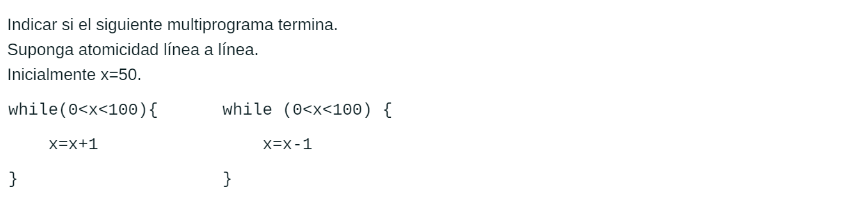
\includegraphics[width=0.9\textwidth]{ps/p7.png}
\begin{rta}
    Puede ocurrir el escenario en donde el planificador, cambia de manera intercalada entre ambos procesos permitiendo a cada uno ejecutar una iteración y así continuar indefinidamente ya que al no aumentar x, \textbf{nunca vamos a poder hacer fallar a la guarda} del while. 
\end{rta}
% ---------------------------------------------------------------------------------- %
% --------------------------- Ejercicio 3 del parcial 2020 --------------------------- %
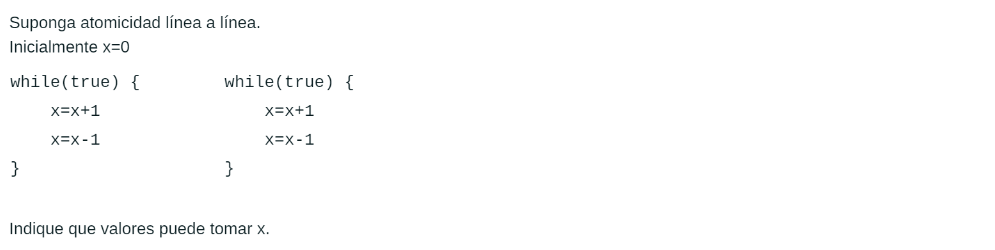
\includegraphics[width=0.9\textwidth]{ps/p8.png}

\begin{rta}
    Para ver cuales de las opciones son posibles, planteo distintos escenarios para cada uno de los valores posibles de las variables.
    \begin{itemize}
        \item \textbf{Valor final 0:} \texttt{A-B-C-1-2-3},
        \item \textbf{valor final 1:} \texttt{A-B},
        \item \textbf{valor final 2:} \texttt{A-B-1-2}
    \end{itemize}
\end{rta}
% ---------------------------------------------------------------------------------- %
% --------------------------- Ejercicio 6 del parcial 2020 --------------------------- %
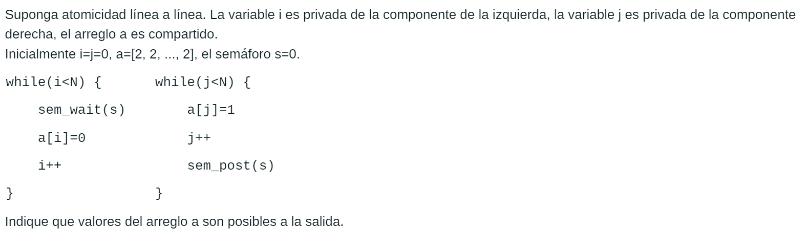
\includegraphics[width=0.9\textwidth]{ps/p11.png}

\begin{rta}
    El semáforo comienza en 0, luego el único proceso que va a poder entrar a tocar el arreglo va a ser el segundo, ya que el primero va a quedar esperando hasta que el segundo lo libere. Primero va a entrar y establecer el valor de la posición en 1, luego entra en el primer proceso y lo establece en 0, así al final el valor que tomará el arreglo es el de \textbf{todas sus componentes en 0}.    
\end{rta}
% ---------------------------------------------------------------------------------- %
% --------------------------- Ejercicio 7 del parcial 2020 --------------------------- %
\newpage
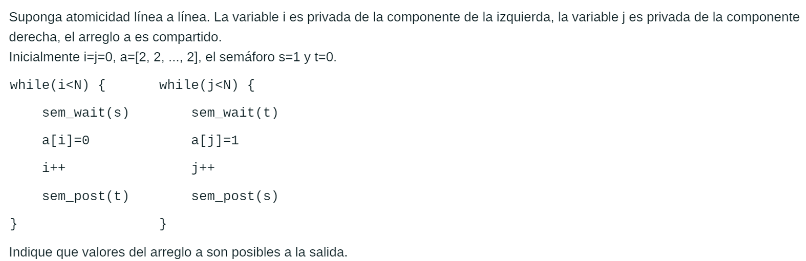
\includegraphics[width=0.9\textwidth]{ps/p13.png}

\begin{rta}
    En este, como el semáforo que comienza en 1 es \texttt{s}, va a empezar el proceso que va a consumir ese recurso que es el primero, establece la posición del arreglo en 0, y despues libera el semáforo para que el segundo proceso pueda entrar y establecer la posición en 1. Al final el arreglo va a tener \textbf{todas sus componentes en 1}.    
\end{rta}
% ---------------------------------------------------------------------------------- %
% --------------------------- Ejercicio 8 del parcial 2020 --------------------------- %
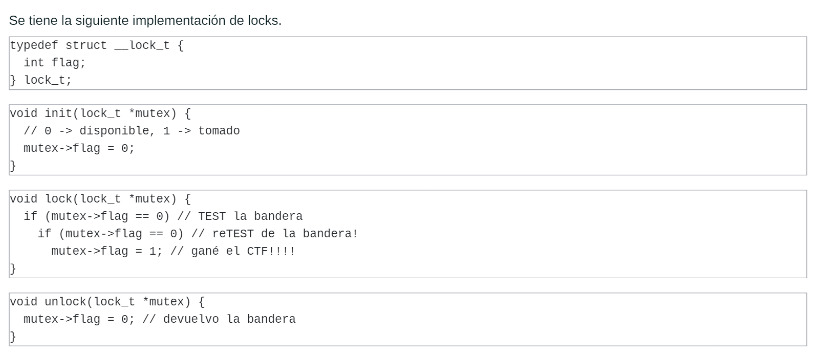
\includegraphics[width=0.8\textwidth]{ps/p12.png}
\begin{rta}
    Va a funcionar a veces, puede ocurrir que ambos entren a ambas guardas de los dos ifs de manera secuencial y así romperse la condición. Al momento de que uno cambie el flag el otro ya pasó la guarda, por lo que ambos entrarian a la CS y se genera un problema.
\end{rta}

% ---------------------------------------------------------------------------------- %
% --------------------------- Ejercicio 12 del parcial 2020 --------------------------- %
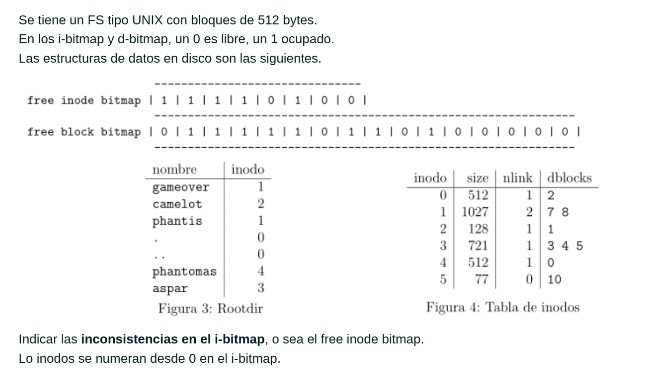
\includegraphics[width=0.9\textwidth]{ps/p5.jpeg}

\begin{rta}
    \begin{itemize}
        \item \textbf{(Inodo 4)} El i-node 4 tiene bloques ocupados y un link, aún así en el bitmap aparece como libre el inodo.
        \item \textbf{(Inodo 5)} El i-node 5 no tiene links es decir sería algo \textit{vacío}, pero en el bitmap aparece como ocupado.
    \end{itemize}    
\end{rta}

% ---------------------------------------------------------------------------------- %

\section*{Ejercicios Segundo Parcial 2021}
% --------------------------- Ejercicio 8 del parcial 2021 --------------------------- %
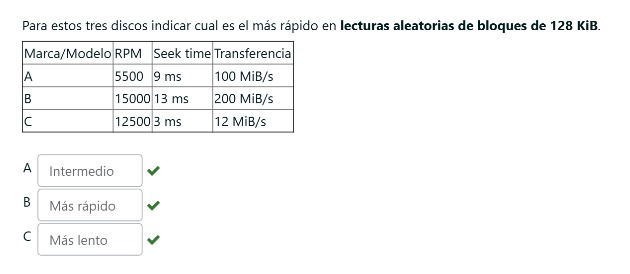
\includegraphics[width=0.7\textwidth]{ps/p4.jpg}

\begin{rta}
    \begin{itemize}
        \item[(A)] \textbf{Intermedio}
        \begin{align*}
            T_{I/O} &= T_{\text{seek}} + T_{\text{rotacional}} + T_{\text{transfer}} \\
            &= 9 + \left( \frac{60}{5500} \cdot 1000  \right)/2 + \frac{128 \cdot 1024}{100 \cdot 2^{20}} \cdot 1000 \\
            &= 9 + 5.45 + 1.25 = 15.7 \\
        \end{align*}
        \item[(B)] \textbf{Más rápido}
        \begin{align*}
            T_{I/O} &= T_{\text{seek}} + T_{\text{rotacional}} + T_{\text{transfer}} \\
            &= 13 + \left( \frac{60}{15000} \cdot 1000  \right)/2 + \frac{128 \cdot 1024}{200 \cdot 2^{20}} \cdot 1000 \\
            &= 13 + 2 + 0.625 = 15.625 \\
        \end{align*} 
        \item[(B)] \textbf{Más lento}
        \begin{align*}
            T_{I/O} &= T_{\text{seek}} + T_{\text{rotacional}} + T_{\text{transfer}} \\
            &= 3 + \left( \frac{60}{12500} \cdot 1000  \right)/2 + \frac{128 \cdot 1024}{12 \cdot 2^{20}} \cdot 1000 \\
            &= 3 + 2.4 +  10.41 = 15.81 \\
        \end{align*}
    \end{itemize}    
\end{rta}
% ---------------------------------------------------------------------------------- %

\section*{Ejercicios Segundo Parcial 2023}
%  --------------------------- Ejercicio 1 del parcial 2023 --------------------------- %
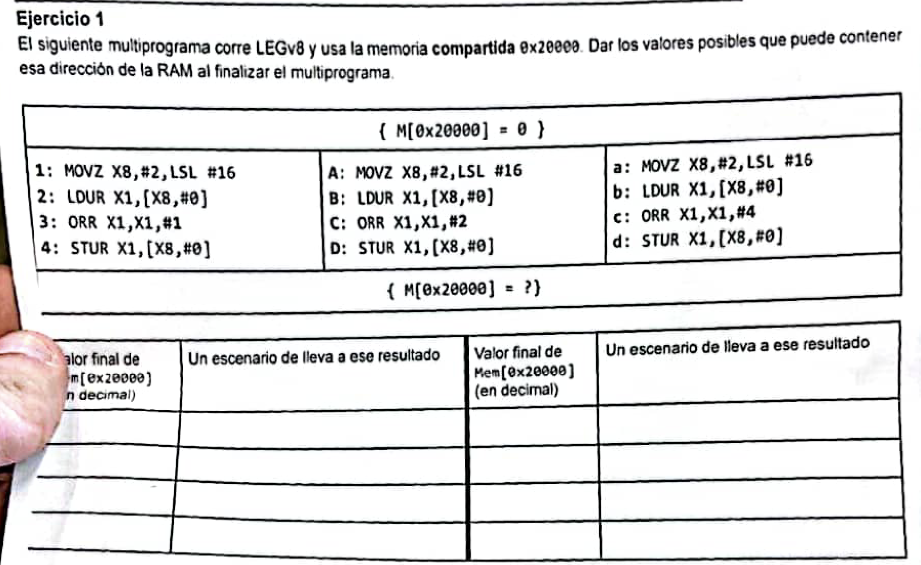
\includegraphics[width=0.8\textwidth]{ps/p1.png}

\begin{rta}
    El código de assembly hace lo siguiente:
    \begin{center}
        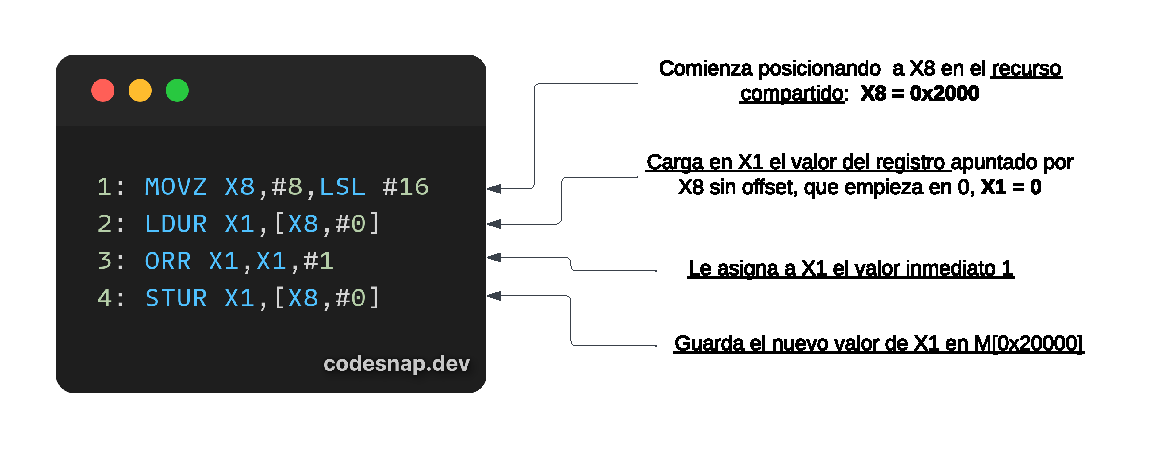
\includegraphics[width=0.8\textwidth]{ps/p2.pdf}    
    \end{center}
    Cabe destacar que en cada cambio de contexto, la función \texttt{switch} va a guardar los registros del proceso en salida y restaurar los actuales con los del proceso que va a entrar, por lo tanto no hay que tener en cuenta el caso de que un registro cambie el valor del mismo pero en otro programa.
    \begin{itemize}
        \item \textbf{Valor final 1:} \texttt{1-2-3-A-B-C-D-a-b-c-d-4}
        \item \textbf{Valor final 2:} \texttt{A-B-C-1-2-3-4-a-b-c-d-D}
        \item \textbf{Valor final 3:} \texttt{A-B-C-D-1-2-3-a-b-c-d-4}
        \item \textbf{Valor final 4:} \texttt{a-b-c-1-2-3-4-A-B-C-D-d}
        \item \textbf{Valor final 5:} \texttt{a-b-c-d-1-2-3-A-B-C-D-4}
        \item \textbf{Valor final 6:} \texttt{a-b-c-d-A-B-C-1-2-3-4-D}
        \item \textbf{Valor final 7:} \texttt{a-b-c-d-1-2-3-4-A-B-C-D}
    \end{itemize}
\end{rta}
% ---------------------------------------------------------------------------------- %
% --------------------------- Ejercicio 2 del parcial 2023 --------------------------- %
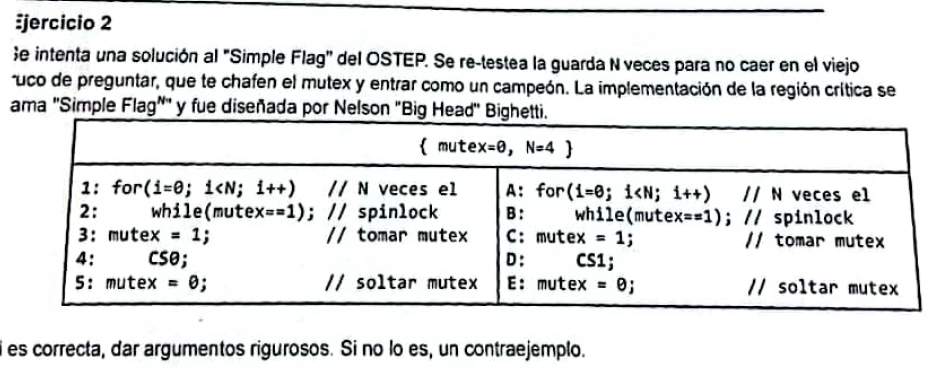
\includegraphics[width=0.8\textwidth]{ps/p2.png}

\begin{rta}    
    El contrajemplo sería el siguiente:
    \begin{enumerate}
        \item Empieza ejecutandose el \textbf{proceso 1} \texttt{N} veces, hace 1-2-1-2-1-2-1-2, luego hace \textbf{context switch} al proceso 2.
        \item Se ejecuta \texttt{N} veces A-B-A-B-A-B-A-B.
        \item Los dos procesos cuando se planifiquen van a \textbf{entrar a la zona crítica sin que se excluyan.}
    \end{enumerate}
    Entonces la solución \textbf{no funciona}.
\end{rta}

% ---------------------------------------------------------------------------------- %
% --------------------------- Ejercicio 3 del parcial 2023 --------------------------- %
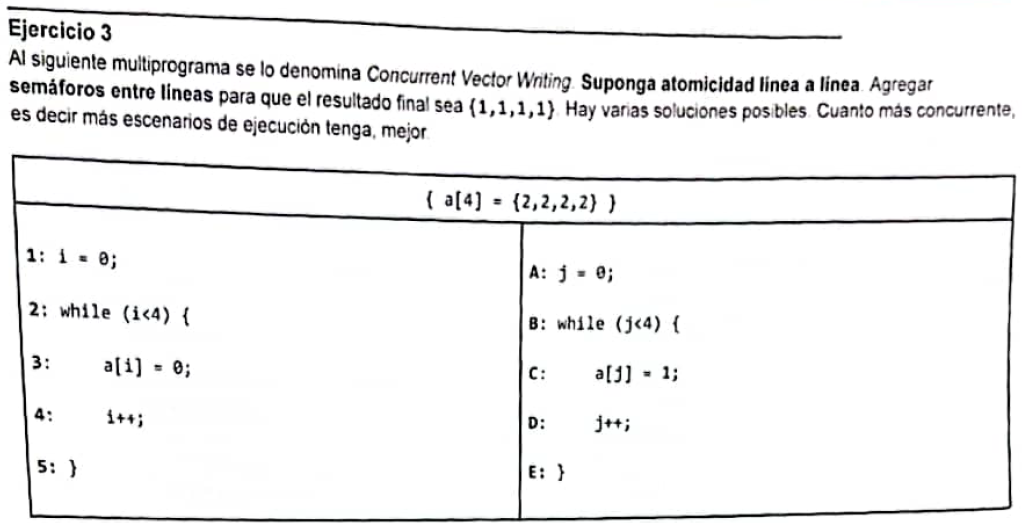
\includegraphics[width=0.8\textwidth]{ps/p3.png}

\begin{rta}
    Una posible solución a esto seria implementar el siguiente manejo de sección crítica: \newline
    \hrule
    \begin{lstlisting}[language=C]
        // Inicializacion
        sem_init(&s1, 0);
    \end{lstlisting}
    \hrule
    \begin{minipage}{0.49\textwidth}
\begin{lstlisting}[language=C]
1: i = 0;
2: while (i<4) {
3:     a[i] = 0;
       sem_post(&s1);
4:     i++;
5: }
\end{lstlisting}
    \end{minipage}
    \begin{minipage}{0.49\textwidth}
\begin{lstlisting}[language=C]
A: j = 0;
B: while (j<4) {
       sem_wait(&s1);
C:     a[j] = 1;
D:     j++;
E: }
\end{lstlisting}
    \end{minipage}

\end{rta}

% ---------------------------------------------------------------------------------- %
\section*{Ejercicios Final 2024-02-09}

% --------------------------- Ejercicio 6 del final 2024-02-09 --------------------------- %
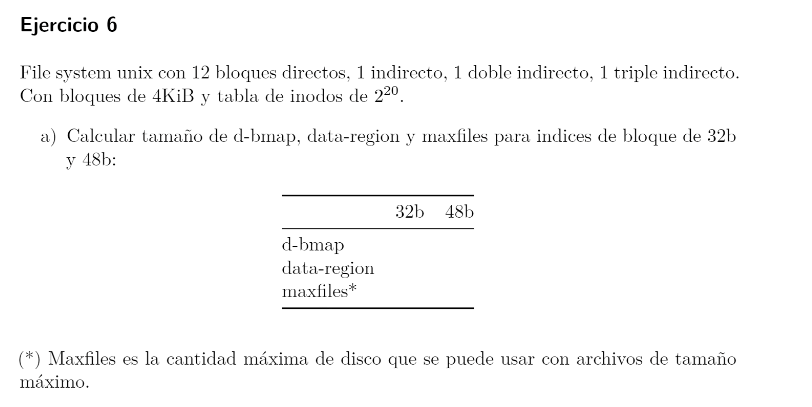
\includegraphics[width=0.8\textwidth]{ps/p15.png}

\begin{rta}
    \begin{itemize}
        \item \textbf{Tamaño del data-bitmap}: Tenemos un bit por cada bloque, si tenemos un índice de bloque de 32b, podemos referenciar $2^{32}$ bloques y por lo tanto el data bitmap va a tener $2^{32}$ bits. De igual manera si tenemos 48 bits, el bitmap va a tener $2^{48}$ bits.
        \item \textbf{Tamaño de la región de datos:} Si cada bloque ocupa 4KiB, entonces la región de datos va a tener $2^{32} \cdot 4KiB = 2^{32} \cdot 2^{12} = 2^{44}$ bytes. En el otro caso donde hay $2^{48}$ bloques, la región de datos va a tener $2^{48} \cdot 4KiB = 2^{48} \cdot 2^{12} = 2^{60}$ bytes.
        \item \textbf{Cantidad máxima de disco con archivos de tamaño máximo:} Buscamos que cada inodo tenga un archivo del tamaño máximo, entonces hay que hallar algo de la forma $2^{20} \cdot \text{maxSize}$:
        \begin{align*}
            \text{maxSize} &= \underbrace{4KiB \cdot 12}_{b-directo} + \underbrace{4KiB \cdot \frac{4069}{4}}_{b-indirecto} + \underbrace{4KiB \cdot \left( \frac{4096}{4} \right)^2}_{b-doble-indirecto} + \underbrace{4KiB \cdot \left( \frac{4096}{4} \right)^3}_{b-triple-indirecto} \\
                           &= 4KiB (12 + 1024 + 1024^2 + 1024^3) \approx 4KiB \cdot 1024^3 = 2^12 \cdot 2^{30} = 2^{42} \\
            \text{maxfiles*} &= 2^{20} \cdot 2^{42} = 2^{62}             
        \end{align*}
        De manera análoga se calcula cuando se tienen 48 bits para el índice de bloque.
    \end{itemize}
\end{rta}
% ---------------------------------------------------------------------------------- %

% --------------------------- Ejercicio 3 del final 2024-02-09 --------------------------- %
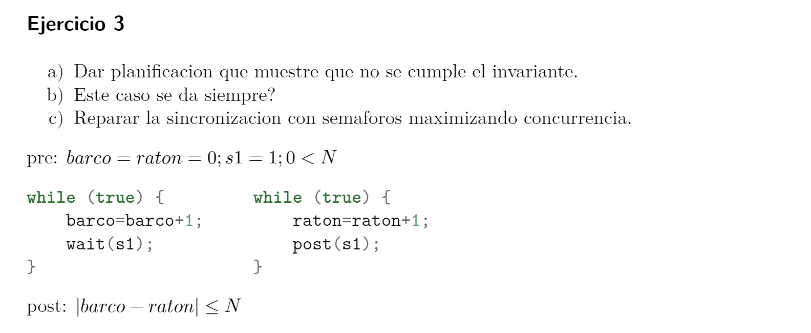
\includegraphics[width=0.86\textwidth]{ps/p16.png}

\begin{rta}
    \begin{itemize}
        \item[(a)] \textbf{Planificación que no cumple el invariante:} el raton se incrementa N+2 veces y el barco 1 vez, ahi el invariante ya no se cumple ya que barco - raton va a ser mayor a N.
        \item[(b)] \textbf{Ese caso no se da siempre}, todo depende del planificador.
        \item[(c)] \textbf{Sincronización:} \newline
        \begin{minipage}{0.49\textwidth}
    \begin{lstlisting}[language=C]
        while(true) {
            barco = barco + 1;
            wait(s1);
            post(s2);
        }
    \end{lstlisting}
        \end{minipage}
        \begin{minipage}{0.49\textwidth}
    \begin{lstlisting}[language=C]
        while(true) {
            wait(s2);
            raton = raton + 1;
            post(s1);
        }
    \end{lstlisting}
        \end{minipage}
    \end{itemize}
\end{rta}
% ---------------------------------------------------------------------------------- %

% --------------------------- Ejercicio 4 del final 2024-02-09 --------------------------- %
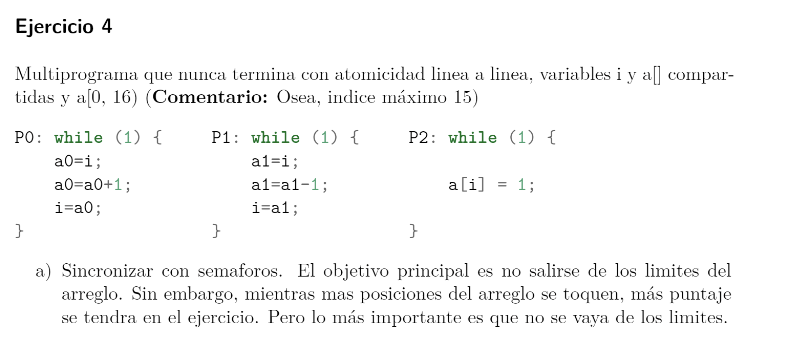
\includegraphics[width=0.82\textwidth]{ps/p17.png}

\begin{rta}
    Una posible solución sería:
    \newline
    \hrule
\begin{lstlisting}[language=C]
// Inicializacion
sem_init(&s1, 0);
sem_init(&s2, 0);
sem_init(&s3, 1);
\end{lstlisting}
    \hrule
    \begin{minipage}{0.32\textwidth}
\begin{lstlisting}[language=C]
    P0: while(1) {
        sem_wait(&s1);
        a0 = i;
        a0 = a0 + 1;
        i = a0;
        if ( i >= 0 ) {
            sem_post(&s3);
        }
        if ( i < 0 ) {
            sem_post(&s1);
        }
    }
\end{lstlisting}
    \end{minipage}
    \begin{minipage}{0.32\textwidth}
\begin{lstlisting}[language=C]
    P1: while(1) {
        sem_wait(&s2);
        a1 = i;
        a1 = a1 - 1;
        i = a1;
        if ( i == 0 ) {
            sem_post(&s3);
        }
        if ( i > 0 ) {
            sem_post(&s2);
        }
    }
\end{lstlisting}
    \end{minipage}
    \begin{minipage}{0.32\textwidth}
\begin{lstlisting}[language=C]
    P2: while(1) {
        sem_wait(&s3);
        if ( i < 0 ){
            sem_post(&s1);
            sem_wait(&s3);
        }
        if ( i > 15 ) {
            sem_post(&s2);
            sem_wait(&s3);
        }
        a[i] = 1;
        sem_post(&s1)
    }
\end{lstlisting}
    \end{minipage}
    \hrule
    \begin{itemize}
        \item Comienza siempre ejecutandose P2 que es el encargado de modificar las posiciones del arreglo. 
        \begin{enumerate}
            \item Si el índice es negativo, está fuera de los límites, por lo que libera el lock del P0, para que este incremente hasta que llegue a 0 y una vez llega, vuelve a liberar el lock, el proceso 0, va a incrementar el i, y \textbf{se va a autoliberar el lock para poder funcionar en bucle mientras sea negativo}. Y una vez que llegue a 0, el proceso 0 libera el lock para que el proceso 2 pueda seguir y se bloquea hasta que alguien lo libere.
            \item Si el índice es mayor a 15, está fuera de los límites, el proceso 2 va a liberar el lock del proceso 1, para que este \textbf{decremente} hasta que llegue a 0, luego libera el lock para que el proceso 2 pueda seguir y se bloquea hasta que alguien lo libere. Solamente se \textbf{autolibera} mientras el índice sea mayor a 0, forzando a que el proceso 1 \textbf{decremente hasta llegar a 0}.
            \item Mientras no se salga de los límites simplemente se libera el lock del proceso 0 para que este pueda seguir incrementando el índice.
        \end{enumerate}
    \end{itemize}
\end{rta}
% ---------------------------------------------------------------------------------- %
\newpage
% --------------------------- Ejercicio 5 del final 2024-02-09 --------------------------- %
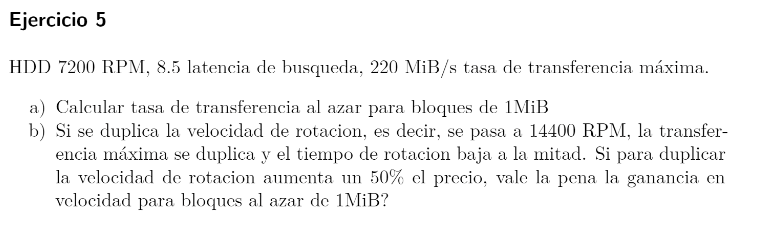
\includegraphics[width=0.82\textwidth]{ps/p18.png}

\begin{rta}
    \begin{itemize}
        \item[(a)] \textbf{Tasa de transferencia al azar de 1MiB:}
        \begin{align*}
            T_{\text{I/O}} &= T_{\text{seek}} + T_{\text{rotacional}} + T_{\text{transfer}} \\
                           &= 8.5 + \left( \frac{60}{7200} \cdot 1000  \right)/2 + \frac{1 \cdot 2^{20}}{220 \cdot 2^{20}} \cdot 1000 = 17.21 \\
            R_{\text{I/O}} &= \frac{1 \cdot 2^{20}}{17.21} = 60928,2975 KiB                   
        \end{align*}
        \item [(b)] Con los datos nuevos sería:
        \begin{align*}
            T_{\text{I/O}} &= 8.5 + \left( \frac{60}{14400} \cdot 1000  \right)/2 + \frac{1 \cdot 2^{20}}{440 \cdot 2^{20}} \cdot 1000 = 12.85 \\
            R_{\text{I/O}} &= \frac{1 \cdot 2^{20}}{12.85} = 81601.24514 KiB
        \end{align*}
        No vale la pena, tomando precios arbitrarios, terminas ganando mas con el disco de 7200 RPM.
    \end{itemize}
\end{rta}
% ---------------------------------------------------------------------------------- %

\section*{Ejercicios Final 2022-02-25}
% --------------------------- Ejercicio 3 del final 2022-02-25 --------------------------- %
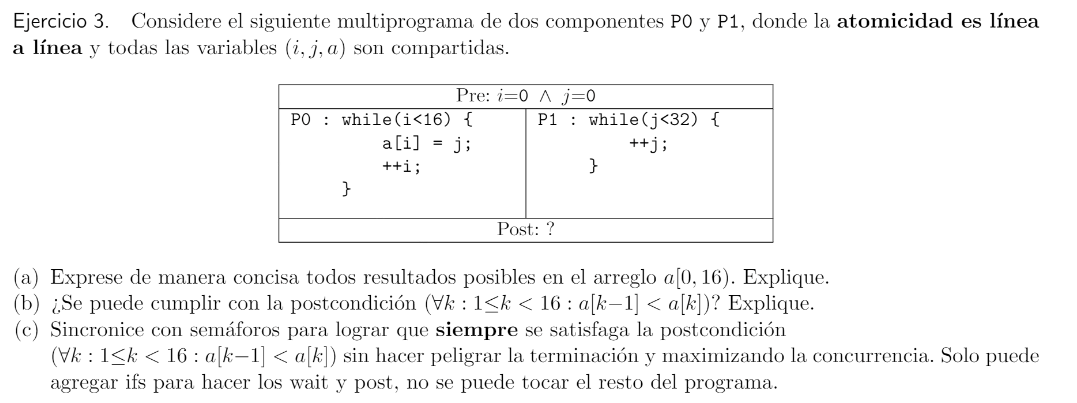
\includegraphics[width=0.94\textwidth]{ps/p19.png}

\begin{rta}
    \begin{itemize}
        \item[(a)] \textbf{Resultados posibles} por como están organizados los programas, yo debería poder plantear el número de formas en las que puedo llenar el arreglo de 16 posiciones con números del 0 al 32, cumpliendo la condición de que:
        \begin{equation*}
            \langle \forall k: 1 \leq k < 16: a[k] \leq a[k+1] \rangle 
        \end{equation*}
        \item[(b)] Sí se puede cumplir esa postcondición, acá hay algunos ejemplos:
        \begin{enumerate}
            \item \textbf{[0,1,2,...,15]} El planificador da lugar a una iteración de cada proceso, comenzando desde el proceso 0.
            \begin{equation*}
                \langle \forall k: 1 \leq k < 16: a[k] = k \rangle 
            \end{equation*}
            \item \textbf{[1,2,3,...,16]} El planificador da lugar a una iteración de cada proceso, comenzando desde el proceso 1.
            \begin{equation*}
                \langle \forall k: 1 \leq k < 16: a[k] = k+1 \rangle 
            \end{equation*}
            \item \textbf{[0,2,4,...,17]} El planificador da lugar a dos iteraciones de cada proceso, comenzando desde el proceso 0.
            \begin{equation*}
                a[0] = 0 \wedge \langle \forall k: 1 < k < 16: a[k] = k+2 \rangle 
            \end{equation*}
        \end{enumerate}
    \end{itemize}
\end{rta}
% ---------------------------------------------------------------------------------- %

% --------------------------- Ejercicio 4 del final 2022-02-25 --------------------------- %
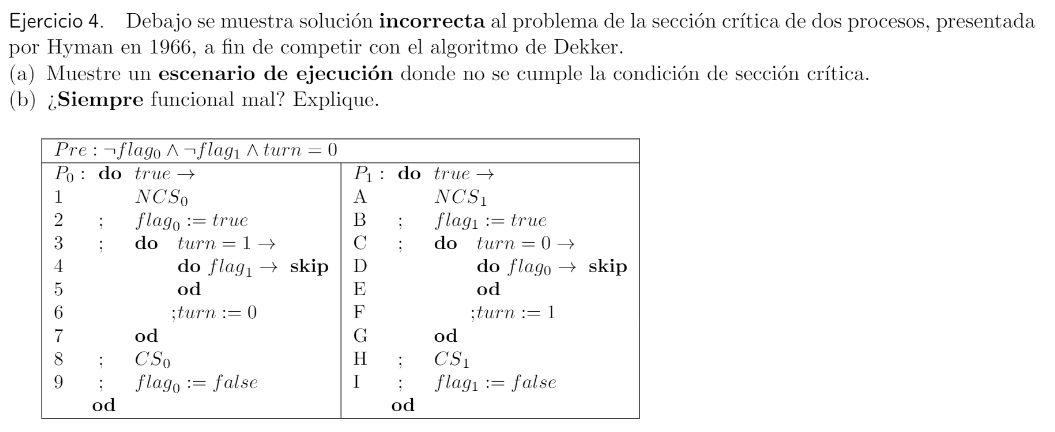
\includegraphics[width=0.97\textwidth]{ps/p20.png}

\begin{rta}
    \begin{itemize}
        \item[(a)] Un posible escenario en el que fallaría es el siguiente:
        \begin{equation*}
            1-A-B-C-D-E-2-3-7-8-F-G-H
        \end{equation*}
        Acá ambos están en la sección crítica al mismo tiempo, por lo que se rompe la exclusión mutua.
        \item[(b)] No siempre funciona mal, el problema está en las asignaciones de los flags que paran al proceso. 
    \end{itemize}
\end{rta}
% ---------------------------------------------------------------------------------- %

% --------------------------- Ejercicio 6 del final 2022-02-25 --------------------------- %
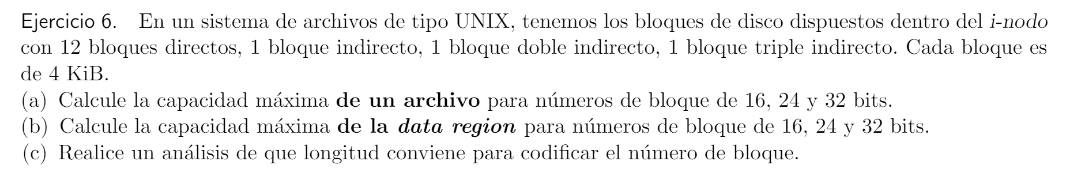
\includegraphics[width=0.97\textwidth]{ps/p21.png}

\begin{rta}
    \begin{itemize}
        \item[(a)] La capacidad máxima de un archivo es aquella que use todos los bloques directos, indirectos, doble indirectos y triple indirectos. Los cálculos son:
        \begin{enumerate}
            \item Con un índice de bloque de 16 bits:
            \begin{align*}
                \text{MaxFileSize} &= \underbrace{4KiB \cdot 12}_{\text{bloque directo}} + \underbrace{4KiB \cdot \frac{4096}{2}}_{\text{bloques indirectos}} + \underbrace{4KiB \cdot \left( \frac{4096}{2} \right)^2}_{\text{bloque doble indirecto}} + \underbrace{4KiB \cdot \left( \frac{4096}{2} \right)^3}_{\text{bloque triple indirecto}} \\
                                   &= 4KiB (12 + 2048 + 2048^2 + 2048^3) \approx 4KiB \cdot 2048^3 = 2^{12} \cdot 2^{33} = 2^{45} = 32TiB
            \end{align*}
            \item Con un índice de bloque de 24 bits:
            \begin{align*}
                \text{MaxFileSize} &= \underbrace{4KiB \cdot 12}_{\text{bloques directos}} + \underbrace{4KiB \cdot \frac{4096}{3}}_{\text{bloques indirectos}} + \underbrace{4KiB \cdot \left( \frac{4096}{3} \right)^2}_{\text{bloque doble indirecto}} + \underbrace{4KiB \cdot \left( \frac{4096}{3} \right)^3}_{\text{bloque triple indirecto}} \\
                                   &= 4KiB (12 + 1365 + 1365^2 + 1365^3) \approx 4KiB \cdot 1365^3 = 2^{12} \cdot 1363^3 = 9.43TiB
            \end{align*}
            \item Con un índice de bloque de 32 bits:
            \begin{align*}
                \text{MaxFileSize} &= \underbrace{4KiB \cdot 12}_{\text{bloques directos}} + \underbrace{4KiB \cdot \frac{4096}{4}}_{\text{bloques indirectos}} + \underbrace{4KiB \cdot \left( \frac{4096}{4} \right)^2}_{\text{bloque doble indirecto}} + \underbrace{4KiB \cdot \left( \frac{4096}{4} \right)^3}_{\text{bloque triple indirecto}} \\
                                   &= 4KiB (12 + 1024 + 1024^2 + 1024^3) \approx 4KiB \cdot 1024^3 = 2^{12} \cdot 2^{30} = 2^{42} = 4TiB
            \end{align*}
        \end{enumerate} 
        \item[(b)] La región de datos está dada por el producto entre la cantidad de bloques referenciados por la cantidad de bloques:
        \begin{enumerate}
            \item Con un índice de bloque de 16 bits:
            \begin{equation*}
                \text{DataRegion} = 2^{16} \cdot 4KiB = 2^{16} \cdot 2^{12} = 2^{28} = 256MiB
            \end{equation*}
            \item Con un índice de bloque de 24 bits:
            \begin{equation*}
                \text{DataRegion} = 2^{24} \cdot 4KiB = 2^{24} \cdot 2^{12} = 2^{36} = 64GiB
            \end{equation*}
            \item Con un índice de bloque de 32 bits:
            \begin{equation*}
                \text{DataRegion} = 2^{32} \cdot 4KiB = 2^{32} \cdot 2^{12} = 2^{44} = 16TiB
            \end{equation*}
            \item[(c)] \textbf{Análisis de la longitud del índice}: en un principio este sistema plantea algo medio absurdo ya que con tantas indirecciones hay un cierto desperdicio pq no tenemos un tamaño de bloque muy grande para poder aprovechar todo a lo que vamos a poder redireccionar, entonces podriamos concluir que simplemente basándonos en la región de datos, el tener \textbf{un índice de 32 bits es suficiente}.
        \end{enumerate} 
    \end{itemize}
\end{rta}
% ---------------------------------------------------------------------------------- %

\section*{Ejercicios Final 2021-12-22}
% --------------------------- Ejercicio 3 del final 2021-12-22 --------------------------- %
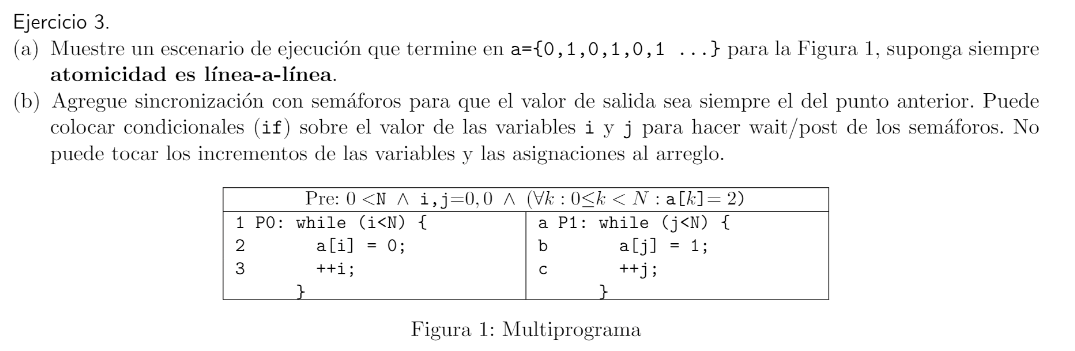
\includegraphics[width=0.97\textwidth]{ps/p22.png}

\begin{rta}
    \begin{itemize}
        \item[(a)] El arreglo comienza con todas sus posiciones en 2, por lo que necesariamente vamos a tener que asignar a cada posición nuevamente para conseguir que se forme el arreglo \texttt{[0,1,0,1,0,1,...]}.
        \begin{equation*}
            a-b-1-2-3-1-2-c-a-b-1-2-3-1-2-c-..
        \end{equation*}
        \item[(b)] La sincronización de los dos procesos puede ser:
        \hrule
\begin{lstlisting}[language=C]
    // Inicializacion
    sem_init(&s1, 1);
    sem_init(&s2, 0);
\end{lstlisting}
        \hrule
        \begin{minipage}{0.48\textwidth}
\begin{lstlisting}[language=C]
P0 : while(i<N) {
        sem_wait(s2) 
        a[i] = 0;
        ++i;
        if(a[j] == 2 )
            sem_post(s2)
        if(a[j] == 0)
            sem_up(s1)
    }
\end{lstlisting}
        \end{minipage}
        \begin{minipage}{0.48\textwidth}
\begin{lstlisting}[language=C]
P1 : while(j<N) {
        sem_wait (s1)
        a[j] = 1;
        ++j; 
        if(a[i] == 2 )
            sem_post(s1)
        if(a[i] == 1)
            sem_up(s2)
}
\end{lstlisting}
        \end{minipage}
        \hrule
    \end{itemize}
\end{rta}
% ---------------------------------------------------------------------------------- %

\section*{Ejercicios varios de Finales}
% --------------------------- Ejercicio 3 del final --------------------------- %

\begin{tcolorbox}[
    colback=blue!20,     % Fondo verde claro
    colframe=blue!60,    % Borde verde
    coltitle=white,       % Color del texto del título
    fonttitle=\bfseries,  % Estilo del título en negrita
    title=Mas ejercicios resueltos de finales,  % Título
    boxrule=1mm,          % Grosor del borde
    rounded corners       % Esquinas redondeadas
]
    \centering
    \href{https://docs.google.com/document/d/1TnR4tz7d3oO_W2JgDb4LBbVTPm8GJsVt6f6tmIMFfSs/edit?usp=sharing}{\textbf{\textcolor{white}{\fboxsep=1pt\fcolorbox{blue!60}{gray!70}{\phantom{\rule{5cm}{0.2cm}} Entrar con cuenta de unc \phantom{\rule{5cm}{1cm}}}}}}
\end{tcolorbox}


\end{document}